\section{力学概述}

{\itshapeCJK
    我们在中学阶段学习的物理,以力学和电学为重点,特别是力学。我们对滑块、小球、圆形轨道等物理模型十分熟悉。但是由于所学知识特别是数学工具的限制,刚刚中学毕业的我们还不能很好地认识力学。在中学阶段,我们通常会认为力学是物理的一个分支,并且由于尚未接触微积分等工具,当时的我们只能考察物体以质点模型为基础的简单运动。实际上,力学研究的对象远不止于此,而且力学和物理学已经沿着完全不同的画风发展一个世纪多了,业已取得了相当丰硕的成果,特别是在工程当中获得了广发的应用。

接下来,让我们从力学的发展史出发,简要地了解一下力学的研究内容、分支以及研究方法。
}

\subsection{力学的发展历史}

力学的内容十分丰富,不是三言两语能够讲清楚的,在概括其发展史时当然也面临这个问题,所以我们接下来的介绍只选择了力学发展中比较重要的主干事件。

\begin{marginparfigure}
    \centering
    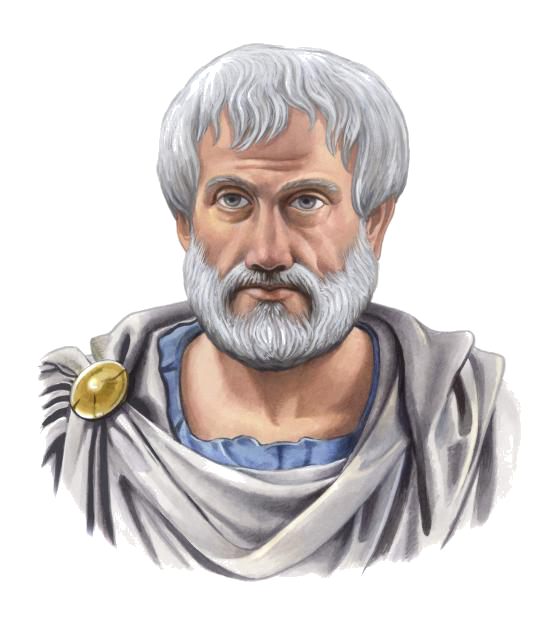
\includegraphics[width = 2.8cm]{Aristotle.png}
    \captionof{figure}{亚里士多德像}
\end{marginparfigure}


\subsubsection{古典时代}

最初,物理学跟力学几乎是同义词。古时候,世界各地的劳动人民就已经在经验上总结许多自然运行的原理,但我们说现代科学的源头在古希腊,因为只有古希腊诞生了形式逻辑与演绎推理,这是数学学科的基础,而一切现代科学又都是建立在形式逻辑、演绎推理与数学描述上的。这里我们介绍一些古希腊时代的著名科学家。

\uwave{亚里士多德}是世界上最伟大的古希腊哲学家与科学家之一,他的研究涉猎广泛,特别是构建了一套影响深远认知系统。尽管亚里士多德的诸多科学结论是错的,却无法掩盖其对现代科学的伟大贡献。


\begin{marginparfigure}
    \centering
    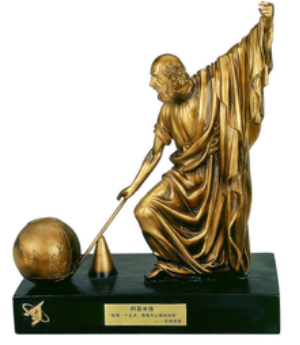
\includegraphics[width = 2.8cm]{Archimedes.png}
    \captionof{figure}{阿基米德像}
\end{marginparfigure}

\uwave{阿基米德}是古希腊最重要的数学家、物理学家之一。一般认为阿基米德是刚体静力学和流体静力学的奠基人,他曾经研究过许多数学和力学问题,如球体积公式、抛物线弓形面积、确定物体重心的方法、物体浮力的计算公式、杠杆原理等。阿基米德曾基于杠杆原理给出一个著名的论断,“给我一个支点,我能撬动地球”。

\begin{marginpartext}
        用如今的观点看,“本轮-均轮模型”是用Fourier级数的方法逼近任意曲线的过程。但若要使逼近足够精确,需要在均轮上添加足够多的“轮上轮”以增加准确性,这正是该体系的繁琐之处。
\end{marginpartext}

此外,阿基米德还制造了许多机械,如螺旋提水机、抛石机等。

\begin{figure}
    \centering
    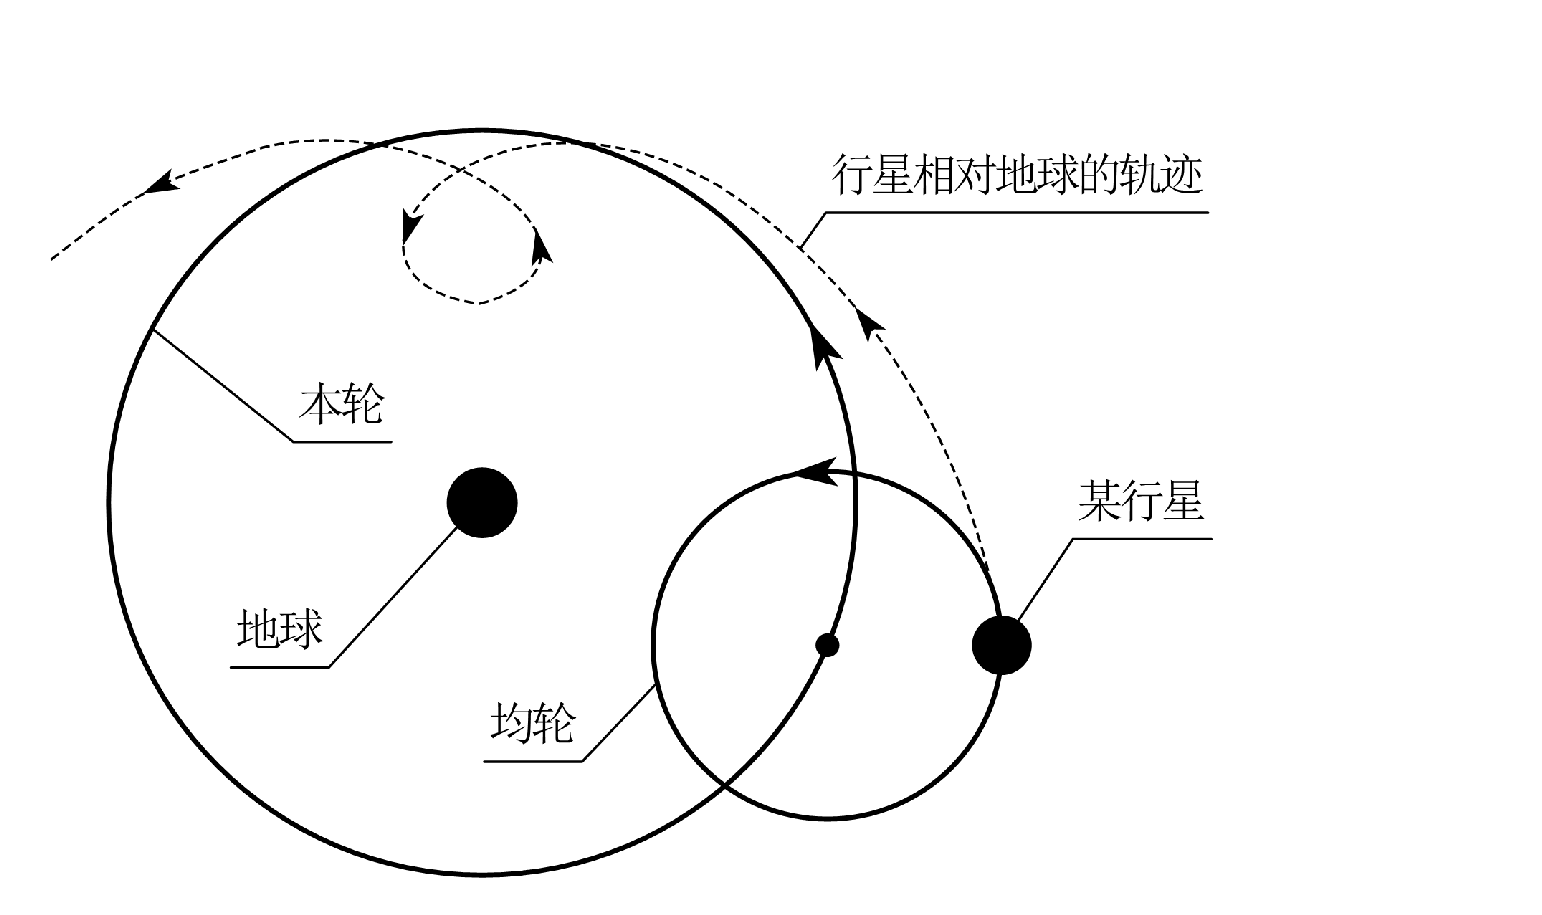
\includegraphics[width = 10.8cm]{epicycle_deferent.pdf}
    \caption{本轮-均轮模型示意}
\end{figure}

古希腊天文学的集大成者是\uwave{托勒密},他认同“地心说”,并且采用\textbf{本轮-均轮模型}来解释行星的运动。托勒密体系的观测精度满足了那个时代的要求,同时“地心说”被认为符合基督教的教义,因而这套体系统治了西方世界1000多年,直到文艺复兴时期才被推翻。

这个时期,由于数学工具还比较初等,微积分等近代数学工具还没出现。尽管阿基米德已经有微积分的思想萌芽,但毕竟不成体系,要系统研究运动学和动力学存在很大困难。所以力学的研究被限制在比较简单的范畴,主要是静力学和比较简单的运动学。

\subsubsection{力学奠基时代}

文艺复兴时期,古希腊的知识得到复兴,各个学科都呈现出一片繁荣景象,新思想和观点的碰撞,使得人们对客观世界的认识有了很大的进步。\uwave{达·芬奇}是文艺复兴时期科学和工程技术领域最重要的人物之一,他提出了许多领先于他那个时代的观点,设计了许多机械图纸,并且还主持修建了诸多水利工程。可以说,达·芬奇揭开了那个科学技术快速发展时代的序幕。

\begin{figure}[ht]
    \centering
    \begin{subfigure}[t]{0.4\textwidth} \centering
        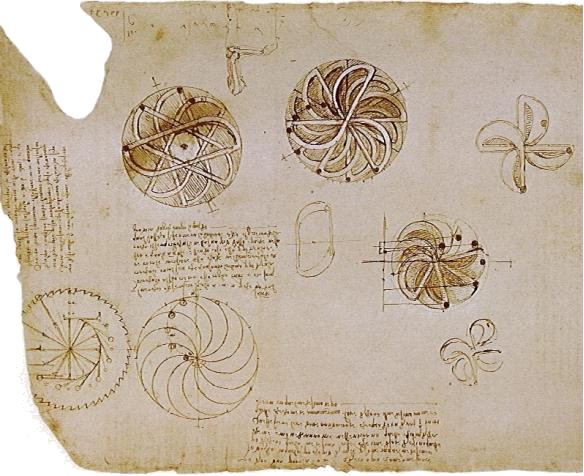
\includegraphics[height = 0.7\linewidth]{daVinci_s.png}
        \caption{达·芬奇的手稿}
    \end{subfigure}\quad
    \begin{subfigure}[t]{0.4\textwidth} \centering
        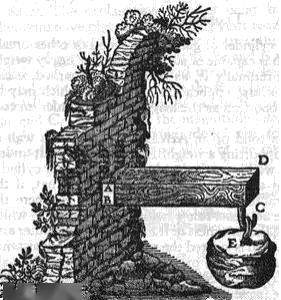
\includegraphics[height = 0.7\linewidth]{Galileo_s_beam.png}
        \caption{伽利略的悬臂梁模型}
    \end{subfigure}\bigskip
\end{figure}



\uwave{伽利略}是“近代科学之父”,
\begin{marginparfigure}
    \centering
    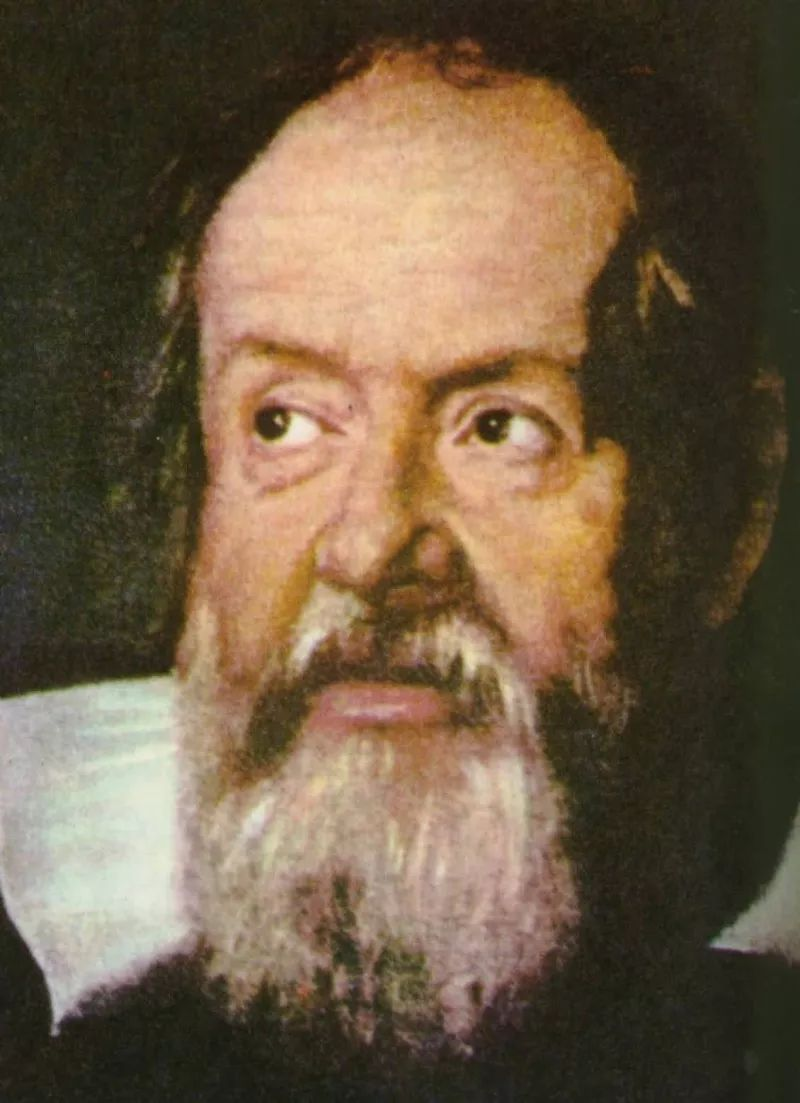
\includegraphics[width = 2.8cm]{Galileo.jpeg}
    \captionof{figure}{伽利略像}
\end{marginparfigure}
他开创了系统科学试验与观察的先河,这种实证精神一直延续到今天的科学研究中。伽利略对于力学和天文学的贡献很大,他首次定量地提出“加速度”的概念,奠定了动力学研究的基础;最早给出了惯性定律;给出了参考系、\textbf{伽利略变换}、相对性原理等概念;另外,伽利略还讨论了悬臂梁变形问题。

\uwave{开普勒}基于其老师第谷的天文观测数据,总结并提出了关于\textbf{行星运动的三大定律},这三条定律为牛顿最终创立经典力学体系奠定了基础。

\begin{figure}[ht]
    \centering
    \begin{subfigure}[t]{0.4\textwidth} \centering
        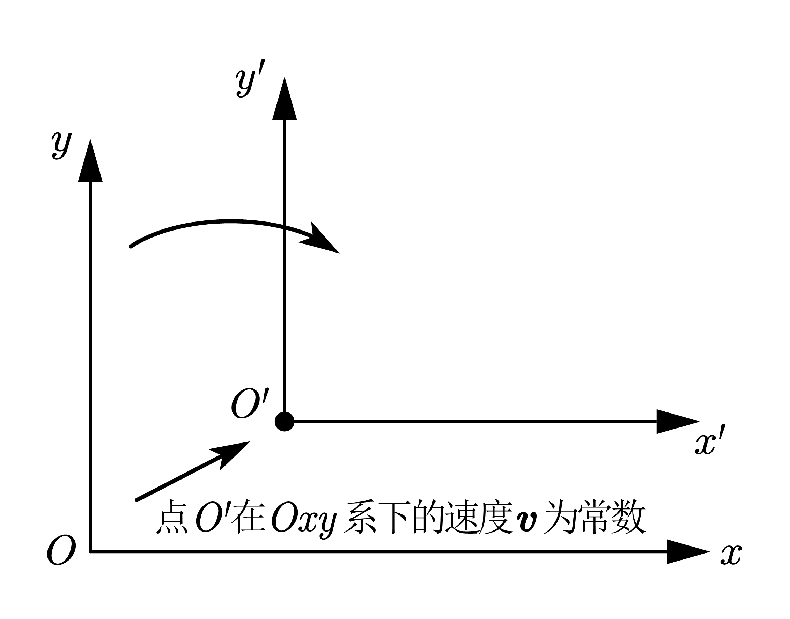
\includegraphics[height = 0.7\linewidth]{Galileo_trans.pdf}
        \caption{伽利略变换}
    \end{subfigure}\quad
    \begin{subfigure}[t]{0.4\textwidth} \centering
        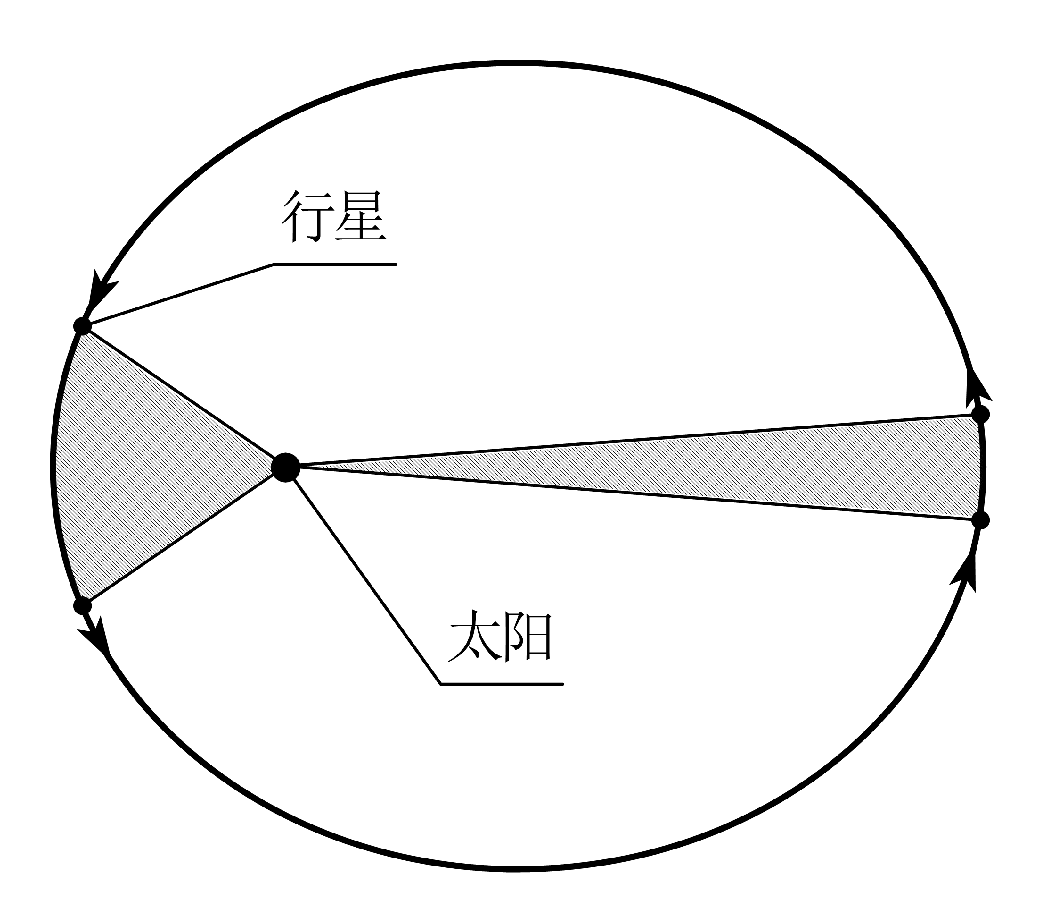
\includegraphics[height = 0.7\linewidth]{Kepler_2.pdf}
        \caption{开普勒第二定律示意}
    \end{subfigure}
\end{figure}

最终创立经典力学体系的工作是由\uwave{牛顿}
\begin{marginparfigure}
    \centering
    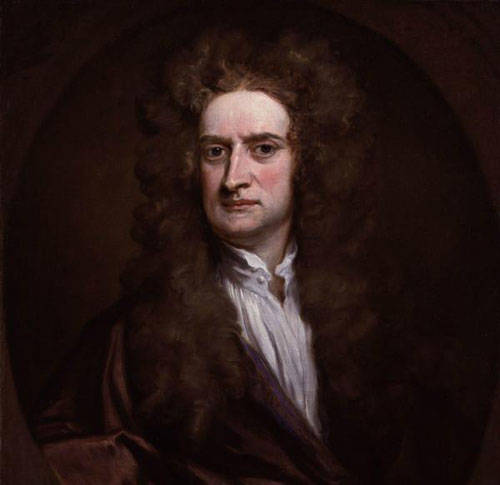
\includegraphics[width = 2.8cm]{Newton.jpg}
    \captionof{figure}{牛顿像}
\end{marginparfigure}在总结前人工作成果的基础上完成的。首先,牛顿总结出了\textbf{牛顿三定律},描述物体运动,这些内容大家十分熟悉,就不再阐述了。其次,牛顿研究了万有引力,最终正确地给出了\textbf{万有引力定律}的数学表达式。牛顿的《自然哲学的数学原理》总结了他所做的大部分力学相关的工作,标志着经典力学体系的成熟。牛顿能取得这些成绩的一个关键因素是他发明并采用了微积分的语言来描述,这是与他同时代许多采用几何观点研究力学的学者所不同的地方。微积分这一数学工具极大地拓展了数学能够描述的物理问题的范围,从这里开始,人们广泛地应用微分方程描述物理规律,再加以求解,成为了定量研究问题的一套范式。

这个时期。还有许多其他著名的学者,如\uwave{惠更斯}、\uwave{胡克}、\uwave{托里拆利}等人,他们在经典力学奠基的阶段也做出了重要的贡献,限于篇幅我们不一一介绍。

\subsubsection{力学进一步发展的时代——分析力学}

接下来力学的发展可以用两条线索概括,其一是经典力学理论进一步发展,得到分析力学体系;其二是对连续介质力学,即固体力学和流体力学的研究。

在牛顿之后,经典力学得到进一步发展。当时的科学家们总结出了诸多定律,守恒定律包括动量、角动量(动量矩)、能量守恒定律;\uwave{达朗贝尔}提出了\textbf{达朗贝尔原理},在非惯性系中添加了“惯性力”,使得能用静力学的手段处理动力学问题;\uwave{约翰·伯努利}首次给出了\textbf{虚功原理}的表述。同时,数学工具得到了进一步发展,对于最速降线问题的讨论导致了变分法这一数学工具的产生,这也标志着分析学正式成为数学的一大分支。


\begin{figure}[ht]
    \centering
    \begin{subfigure}[t]{0.4\textwidth} \centering
        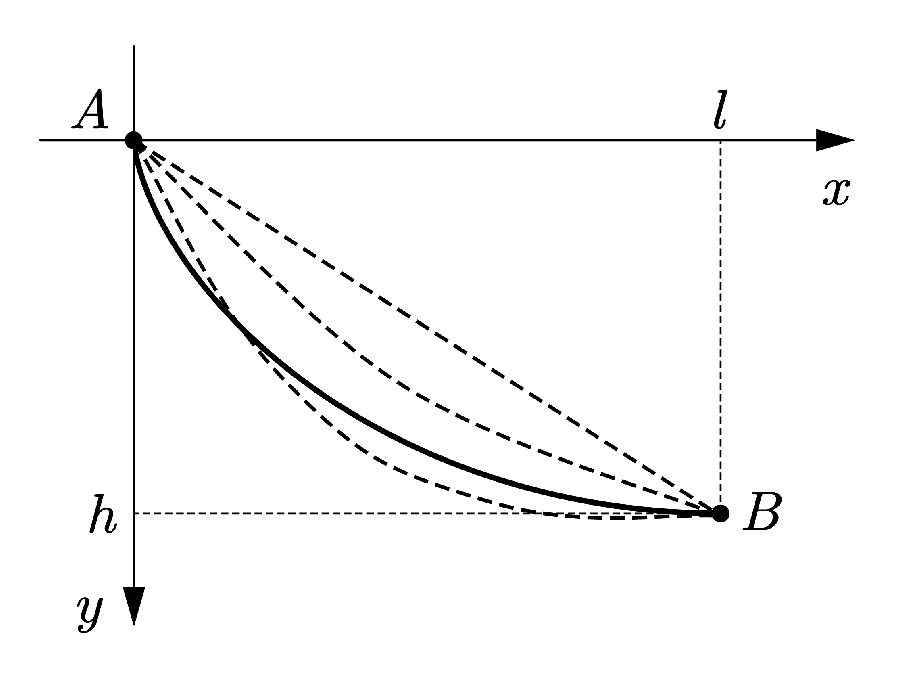
\includegraphics[height = 0.7\linewidth]{cycloid.pdf}
    \end{subfigure}\quad
    \begin{subfigure}[t]{0.4\textwidth} \centering
        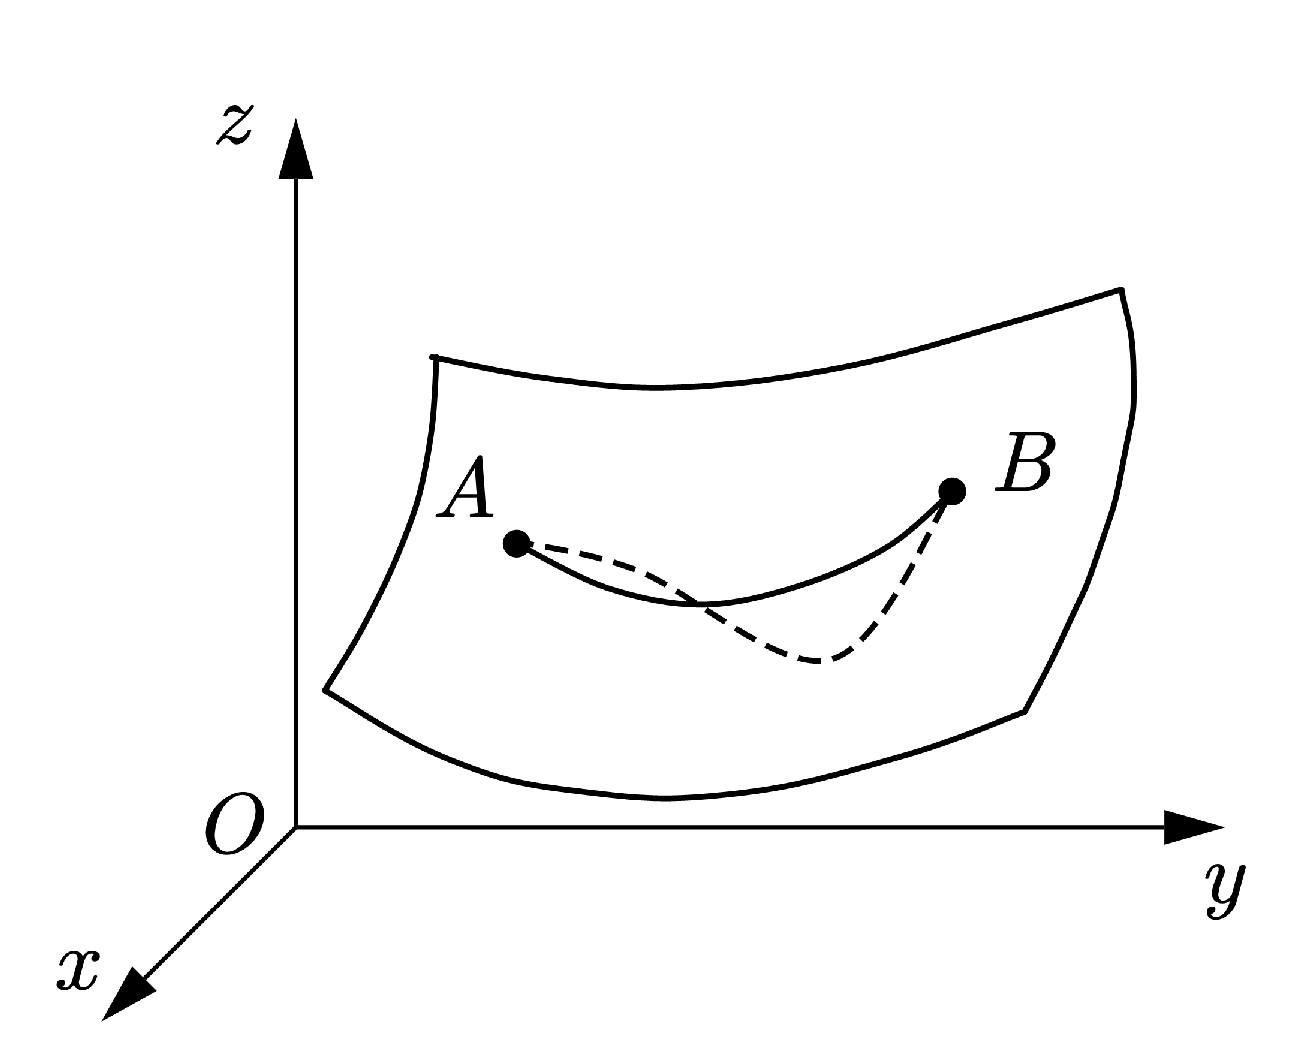
\includegraphics[height = 0.7\linewidth]{geodesic.pdf}
    \end{subfigure}
    \caption{最速降线和曲面短程线问题,对此类泛函极值问题的研究促进了变分法的发展}
\end{figure}
\begin{marginpartext}
    最速降线问题的提法是:设$A$和$B$是铅直平面上不在同一铅直线上的两点,在所有连接$A$和$B$的平面曲线中,求一条曲线,使得仅受重力作用且初速度为零的质点从$A$点沿其运动到$B$点所需时间最短。
\end{marginpartext}

尽管经典力学已经建立起来了,但它还是只能处理简单的质点问题,无法处理刚体(考虑物体的尺寸、形状,并认为物体不会发生变形,与质点相比,存在转动如何描述的问题)这样需要考虑物体形状的问题。同时,牛顿的经典力学理论上能处理有约束的问题,但实际问题过于复杂,用牛顿体系处理并不方便。在这种背景下,分析力学建立起来并得到了发展。

\begin{marginparfigure}
    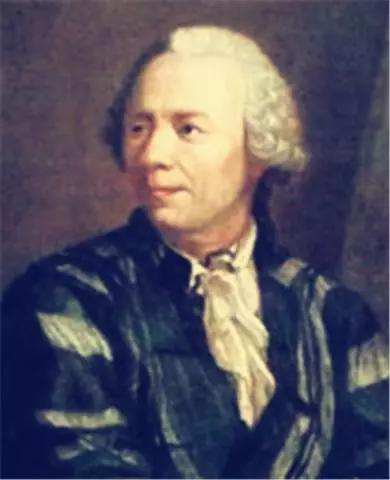
\includegraphics[width = 2.8cm]{Euler.jpg}
    \captionof{figure}{欧拉像}
\end{marginparfigure}

\uwave{欧拉}首先研究了刚体的运动规律,扩大了经典力学能够处理的问题的范畴,而且在这个过程中,产生了\textbf{自由度}的概念,即完整的描述一个力学系统的运动情况所需的最少的变量数。例如,若要完整描述平面刚体的运动速度,只需要知道刚体上任意一点的速度(矢量)及其转动的角速度。自由度的概念是分析力学建立的基础,因而十分重要。此外,欧拉给出了极值曲线、等周问题的解答,创立了变分学,并富有创见性地提出“分析学具有重构牛顿力学体系的潜力”。

\begin{figure}[ht]
    \centering
    \begin{subfigure}[t]{0.4\textwidth} \centering
        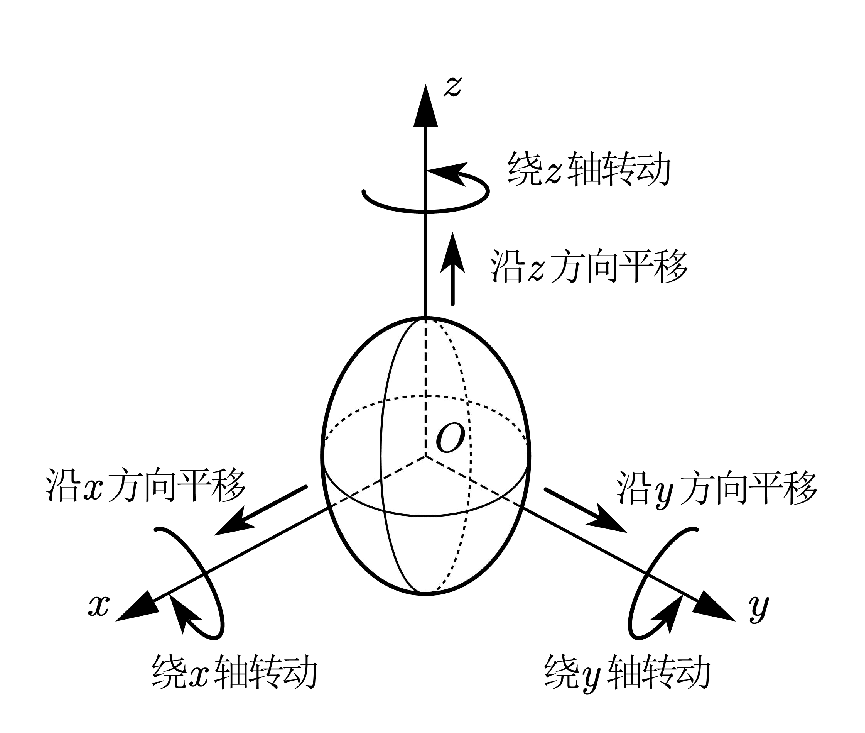
\includegraphics[height = 0.7\linewidth]{freedom.pdf}
    \end{subfigure}\quad
    \begin{subfigure}[t]{0.4\textwidth} \centering
        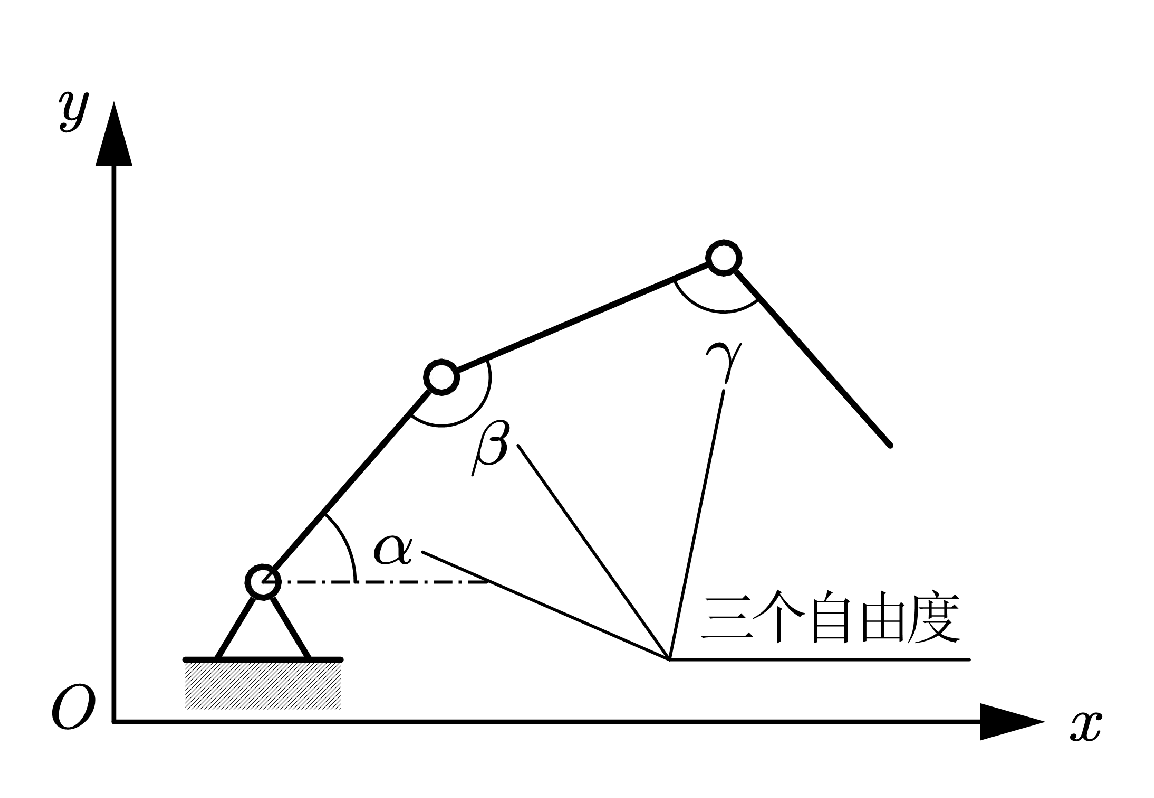
\includegraphics[height = 0.7\linewidth]{machine.pdf}
    \end{subfigure}
    \caption{自由度与约束}
\end{figure}

\uwave{拉格朗日}实现了欧拉的猜想。如果说牛顿力学体系的核心概念是“力”,那么拉格朗日力学体系的核心概念就是“能量”。拉格朗日从牛顿力学出发,结合达朗贝尔原理和虚功原理,推出了\textbf{(第二类)拉格朗日方程}:

\[
    \frac{\mathrm{d}}{\mathrm{d}t}\frac{\partial L}{\partial \dot{q}_i}=0 \quad (i=1,2,\cdots,n)
    .\]

拉格朗日用\textbf{广义坐标}$q_i$来描述物体的空间位置,其中$n$即为自由度数,这时其对时间的导数——广义速度$\dot{q}_i=\dfrac{\mathrm{d} q_i}{\mathrm{d} t}$的概念就不那么直观了。不过,结合坐标和广义坐标之间的关系

\begin{marginparfigure}
    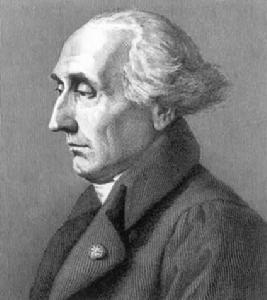
\includegraphics[width = 2.8cm]{Lagrange.jpeg}
    \captionof{figure}{拉格朗日像}
\end{marginparfigure}

\[
    x_j=x_j\left(q_1, q_2, \cdots, q_n\right) \quad \left(j=1, 2, \cdots, N\right)
    .\]

以及偏导数的链式法则,表示出牛顿体系中的物理量还是不困难的。式中的

\[
    L=L(q_1,q_2,\cdots,q_n,\dot{q}_1,\dot{q}_2,\cdots,\dot{q}_n,t)
    .\]

是系统动能与势能之差,我们称之为\textbf{拉格朗日量}。

拉格朗日方程与牛顿的动量定理是等价的,就是说,以二者当中某一个为假设前提,就能推出另一个。拉格朗日体系的数学基础实际上就是变分原理,称
\[
    S=\int_{t_1}^{t_2}{L\,\mathrm{d}t}
    .\]
为\textbf{作用量},当作用量达到极小值(变分等于$0$),就能得到拉格朗日方程。作用量这一概念可以推广到一般的演化系统,只要令某一个演化系统的作用量达到极小值,就能得到一个描述该系统运动规律的方程,这就是\textbf{最小作用量原理}。
\begin{marginpartext}
        牛顿的动量定理指的就是牛顿第二定律,由于$ma$可以写成$\frac{\mathrm{d}p}{\mathrm{d}t}$,其中$p$为动量,这就是动量定理的微分形式,所以有时不区分牛顿第二定律和动量定理。
\end{marginpartext}

拉格朗日体系的高明之处在于回避掉了对复杂约束的讨论,使得问题求解得到简化。然而,拉格朗日体系的好处远不止于此,它虽然是一个和牛顿力学等价的力学体系,但等价不意味着二者完全相等,在分析某些问题时,可能二者当中的某一个更有优势。同时,拉格朗日体系具有更好的泛用性,可以应用在不限于力学的更广泛的问题当中。

\uwave{哈密顿}早期的工作是研究光学,但他将其中的数学方法推广到了力学上,创立了哈密顿力学体系。哈密顿对拉格朗日量$L$进行了勒让德变换
\[
    H\left(q_1,\cdots,q_n,p_1,\cdots,p_n,t\right)=\sum_{i=1}^n{\dot{q}_ip_i}-L\left( q_1,\cdots ,q_n,\dot{q}_1,\cdots ,\dot{q}_n,t \right)
    .\]
其中$p_i$为广义动量。再对该式取变分,就能推出\textbf{哈密顿方程}

\[
    \begin{dcases}
        \dot{q}_i=\dfrac{\partial H}{\partial p_i},  \\
        \dot{p}_i=-\dfrac{\partial H}{\partial q_i}, \\
    \end{dcases} \quad \left( i=1,2,\cdots ,n \right)
    .\]

\begin{marginparfigure}
    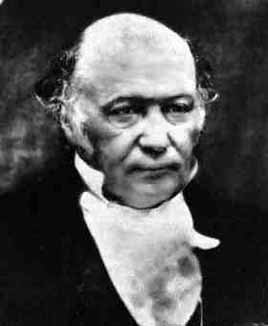
\includegraphics[width = 2.8cm]{Hamilton.jpg}
    \captionof{figure}{哈密顿像}
\end{marginparfigure}

哈密顿推出的方程与拉格朗日的方程和牛顿的运动定律互相等价,但是由于哈密顿的方程具有某种对称性,对于某一类问题的研究和求解来说是很方便的,如量子力学的描述就是基于哈密顿体系的。

这段时期,研究人员注意到所谓守恒律实际上是运动方程的某种积分。\uwave{索菲斯·李}对微分方程进行研究,将微分方程的解与变换群相联系,这使得对微分方程解的研究也可以用到近世代数的手段。\uwave{诺特}进一步提出,作用量的连续对称性意味着守恒。这些思想在日后的物理学研究中发挥着重要的作用。

\subsubsection{力学进一步发展的时代——连续介质力学}

对连续介质力学的研究分为固体力学和流体力学两部分,起初这二者之间没有建立联系,随着研究的逐渐深入,才将它们纳入到一个统一的框架下进行描述。

\begin{marginpartext}
        气体中的激波是这样形成的:气体中扰动产生的波以当地声速进行传播,当扰动源的运动速度超过当地声速时,扰动来不及传播到扰动源前边,这样产生了一个压缩界面,这就是激波。超音速飞行器产生的爆鸣声就是激波导致压强突变产生的。
\end{marginpartext}

对流体的研究比固体的稍早。牛顿在《自然哲学的数学原理》之中,就对流体进行了讨论,提出了“牛顿流体”的概念。之后,\uwave{丹尼尔·伯努利}、欧拉等人建立了不考虑流体粘性的理想流体的动力学方程,但真实流体存在粘性,所以这部分理论只有在粘性可以忽略时才能实用。不过,理想流体动力学的观点和方法论对后序研究是很有价值的。

\uwave{纳维}考虑了流体的粘性,推导出了不可压缩粘性流体的运动方程,稍后,也从连续介质假设出发推导出了这组方程,这就是著名的\textbf{纳维-斯托克斯方程}(N-S方程):

\[
    \frac{\partial(\rho\symbfit{u})}{\partial t}+\nabla\cdot(\rho\symbfit{uu})=\rho\symbfit{f}-\nabla p+\mu\nabla ^2\symbfit{u}
    .\]

在直角坐标系中,将每一项展开就可以写成:
\[
    \begin{dcases}
        \dfrac{\partial v_x}{\partial t}+v_x\dfrac{\partial v_x}{\partial x}+v_y\dfrac{\partial v_x}{\partial y}+v_z\dfrac{\partial v_x}{\partial z}=f_x-\dfrac{1}{\rho}\dfrac{\partial p}{\partial x}+\nu\left(\dfrac{\partial^2 v_x}{\partial x^2}+\dfrac{\partial^2 v_x}{\partial y^2}+\dfrac{\partial^2 v_x}{\partial z^2}\right), \\
        \dfrac{\partial v_y}{\partial t}+v_x\dfrac{\partial v_y}{\partial x}+v_y\dfrac{\partial v_y}{\partial y}+v_z\dfrac{\partial v_y}{\partial z}=f_y-\dfrac{1}{\rho}\dfrac{\partial p}{\partial y}+\nu\left(\dfrac{\partial^2 v_y}{\partial x^2}+\dfrac{\partial^2 v_y}{\partial y^2}+\dfrac{\partial^2 v_y}{\partial z^2}\right), \\
        \dfrac{\partial v_z}{\partial t}+v_x\dfrac{\partial v_z}{\partial x}+v_y\dfrac{\partial v_z}{\partial y}+v_z\dfrac{\partial v_z}{\partial z}=f_z-\dfrac{1}{\rho}\dfrac{\partial p}{\partial z}+\nu\left(\dfrac{\partial^2 v_z}{\partial x^2}+\dfrac{\partial^2 v_z}{\partial y^2}+\dfrac{\partial^2 v_z}{\partial z^2}\right).
    \end{dcases}
\]
这组方程的求解十分困难,以至于时至今日,该组方程光滑解的存在性还没有得到证明。

不可压缩流体的典型便是水,这段时期,得益于不可压缩流体的研究成果日益丰富,水力学和水动力学也得到了发展。许多水利工程、水力机械结合生产经验以及理论分析,获得了许多经验和半经验的公式,大大促进了工程学的发展。

20世纪之前,对于可压缩流体的研究则比较少,主要围绕超声速流动和激波展开,做了基础性的探索。

最早的固体力学来自于对杆、梁、板等变形体的变形、强度、稳定性等问题的研究。早期,伽利略考察过悬臂梁的强度问题;稍晚一些的欧拉考察了梁的小挠度变形(横向变形,即垂直于轴向的变形),以及压杆稳定性问题。

\begin{marginparfigure}
    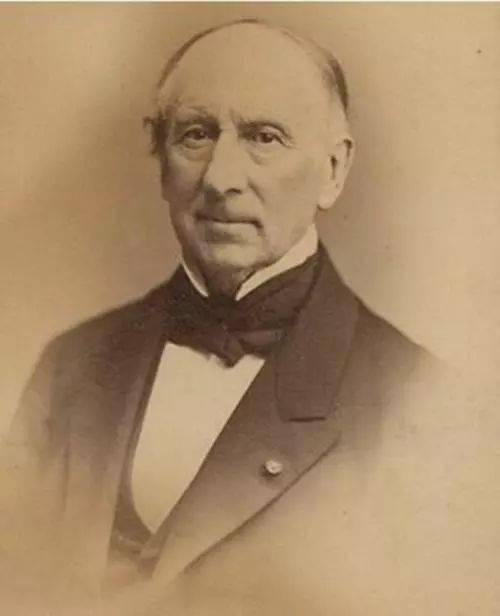
\includegraphics[width = 2.8cm]{Cauchy.jpeg}
    \captionof{figure}{柯西像}
\end{marginparfigure}


随后一段时间,固体力学的研究主要围绕弹性力学展开,这一部分的研究也是比较成熟的。弹性力学理论的先驱是纳维和\uwave{泊松},纳维提出了各向同性弹性体的平衡方程,泊松给出了\textbf{泊松比}的概念。弹性力学理论的奠基者是\uwave{柯西},他引入了\textbf{应变}、\textbf{应力}的概念,讨论了应力应变之间的关系,讨论了平衡微分方程和边界条件的提法,这些内容是线弹性力学的基本内容。

\begin{marginpartext}
        应力描述内力的分布情况,它的量纲与压强相同。

        应变描述变形情况,它的量纲是$1$。

        泊松比描述变形过程中的横向收缩效应。
\end{marginpartext}


\begin{figure}[ht]
    \centering
    \begin{subfigure}[t]{0.8\textwidth} \centering
        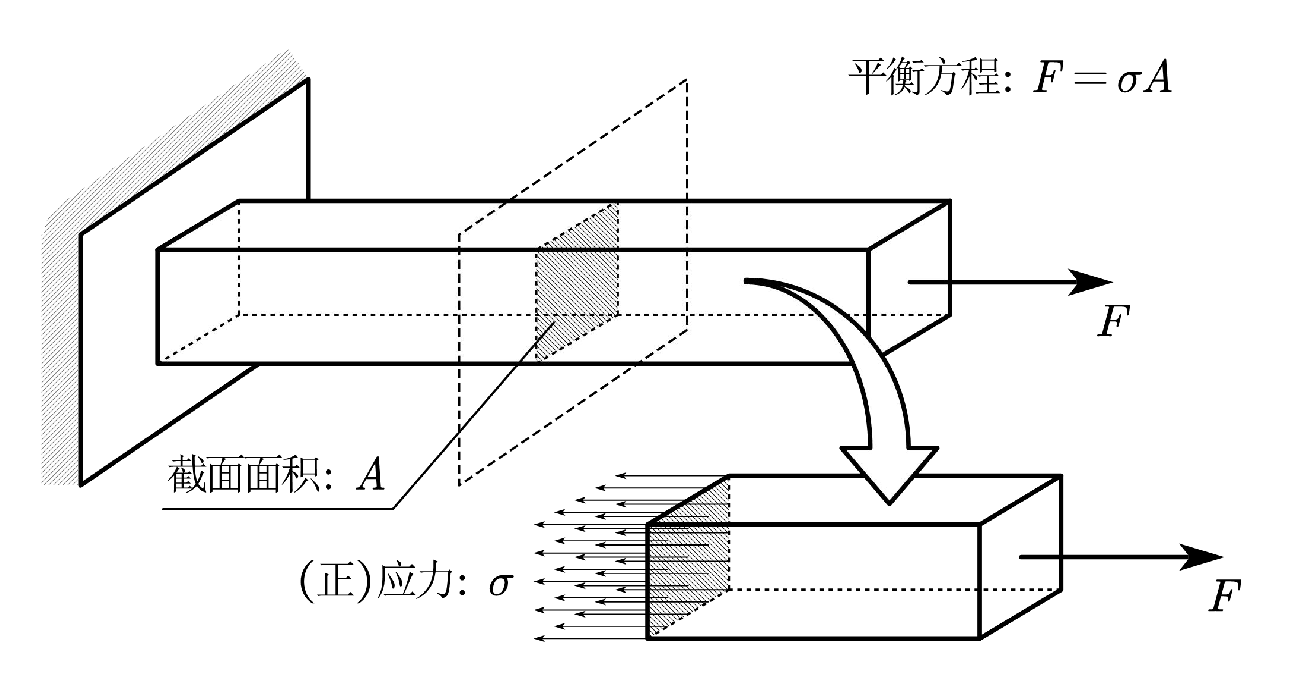
\includegraphics[height = 0.5\linewidth]{stress.pdf}
    \end{subfigure}
    
    \begin{subfigure}[t]{0.8\textwidth} \centering
        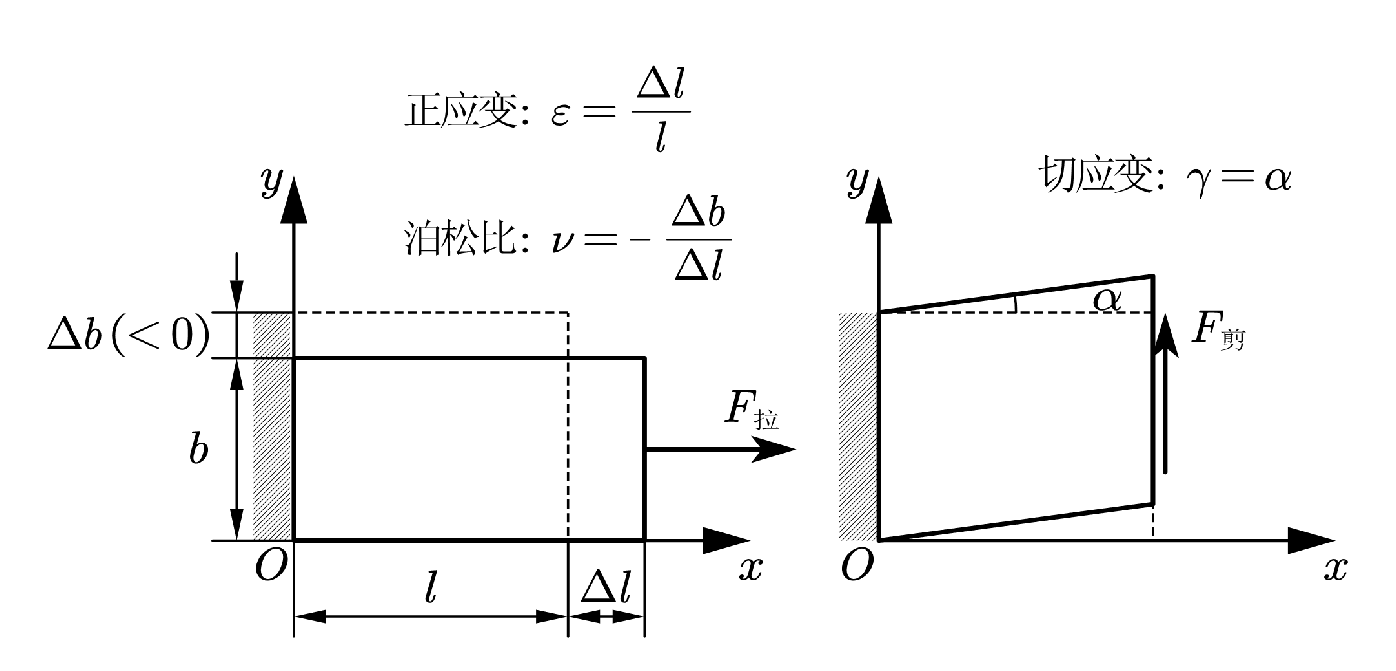
\includegraphics[height = 0.5\linewidth]{strain.pdf}
    \end{subfigure}
    \caption{应力、应变与泊松比}
\end{figure}


\begin{marginparfigure}
    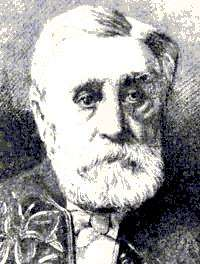
\includegraphics[width = 2.8cm]{Saint_Venant.jpeg}
    \captionof{figure}{圣维南像}
\end{marginparfigure}

建立起弹性力学相关的基本概念后,学者们研究了一些弹性模型的解法。\uwave{圣维南}%
提出了逆解法和半逆解法,是弹性力学求解的重要手段;以及\textbf{圣维南原理},描述了弹性体的局部效应,对于问题求解很有好处。\uwave{柯希霍夫}(基尔霍夫)研究了薄板的理论。\uwave{瑞利}总结了弹性体的振动和声学问题。\uwave{勒夫}总结了前人关于弹性力学的工作,并进一步发展,讨论了薄壳问题,同时还研究了弹性波理论。\uwave{穆斯赫利什维利}致力于用复变函数的手段解析求解弹性力学问题,是计算力学发展之前弹性理论求解的高峰。


\begin{marginpartext}
        复变函数指的是自变量和因变量都是复数的函数,它在描述一些平面问题时具有优势,故在固体力学、流体力学中都有应用。
\end{marginpartext}

\begin{figure}[h]
    \centering
    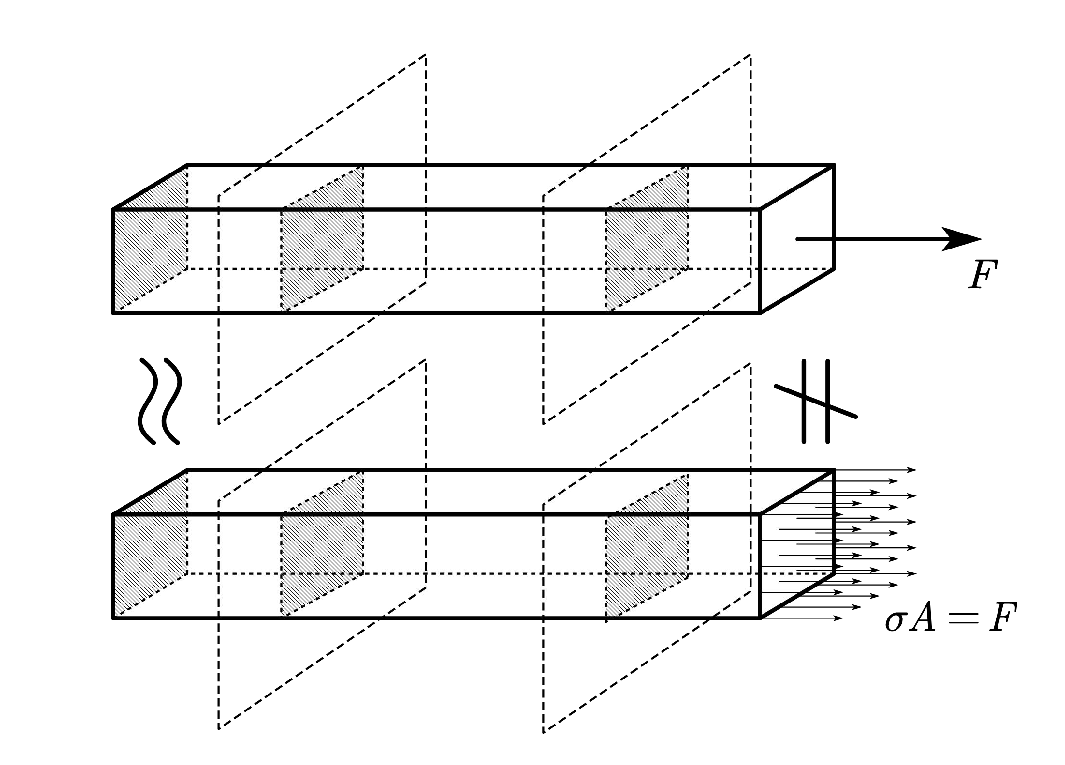
\includegraphics[scale=0.45]{StVenant.pdf}
    \caption{圣维南原理示意}
\end{figure}

弹性力学的发展完善了对\uwave{杆}、\uwave{梁}、\uwave{轴}等基本结构件变形和强度的研究,获得了一些简单且具有工程实用性的结果,这一部分当属材料力学的范畴。同时期,工程上开始结构的变形问题,最典型的是桁架结构和连续梁,并发展了一些求解的方法,这当属结构力学的范畴。此外,由于工程实际的需要和工程事故,人们开始关注疲劳和断裂现象。

\begin{marginpartext}
        一般来说,杆、梁、轴都是细长结构件,区别在于:杆只承受轴向拉压,梁只承受横向外力(弯曲),轴只承受扭转。
\end{marginpartext}

\begin{figure}[ht]
    \centering
    \begin{subfigure}[t]{0.3\textwidth} \centering
        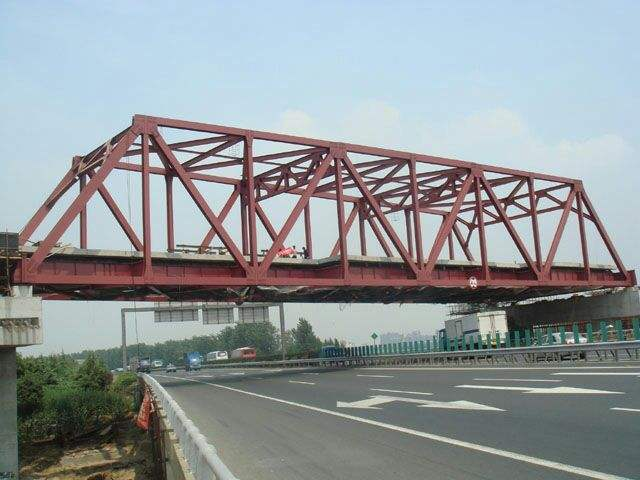
\includegraphics[height = 0.7\linewidth]{truss.jpeg}
        \caption{桁架结构}
    \end{subfigure}\quad
    \begin{subfigure}[t]{0.6\textwidth} \centering
        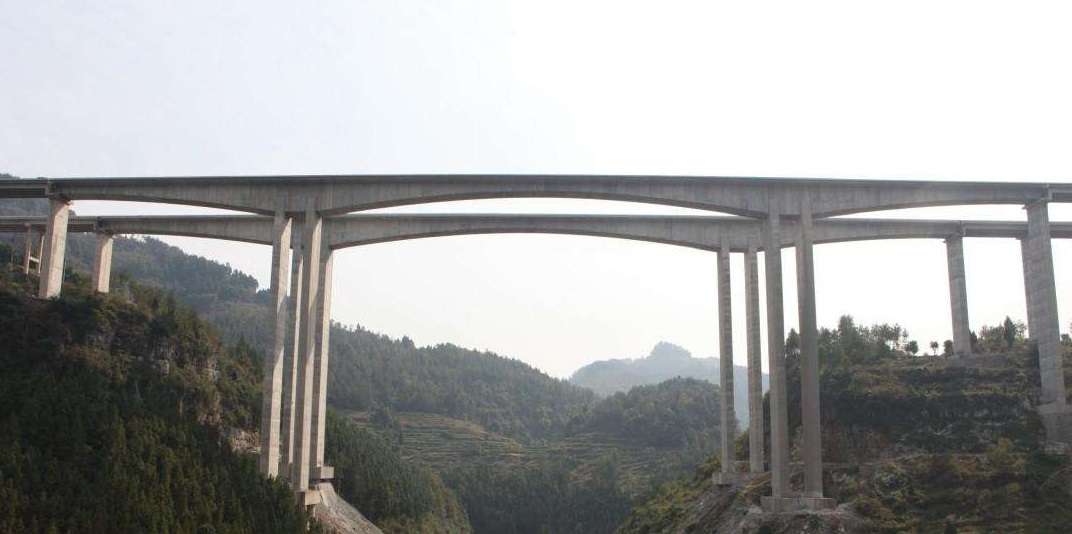
\includegraphics[height = 0.35\linewidth]{continuous_beam.jpeg}
        \caption{连续梁结构}
    \end{subfigure}\bigskip

    \begin{subfigure}[t]{0.8\textwidth} \centering
        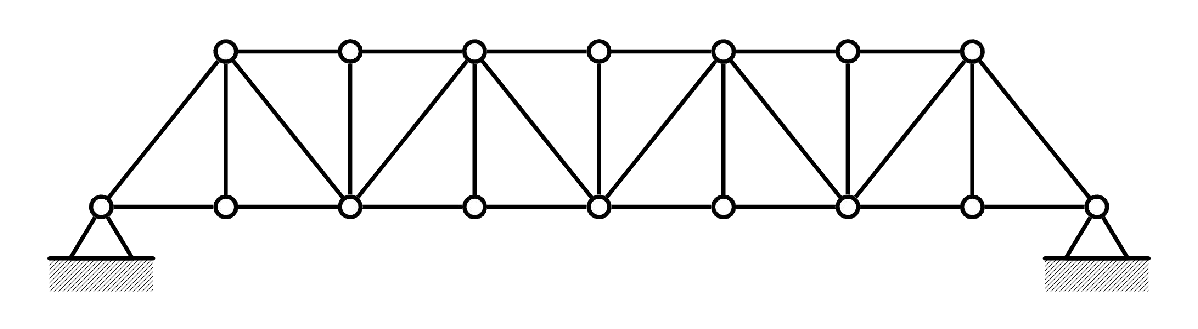
\includegraphics[width = 0.75\textwidth]{truss_model.pdf}
        \caption{桁架模型}
    \end{subfigure}\bigskip

    \begin{subfigure}[t]{0.6\textwidth} \centering
        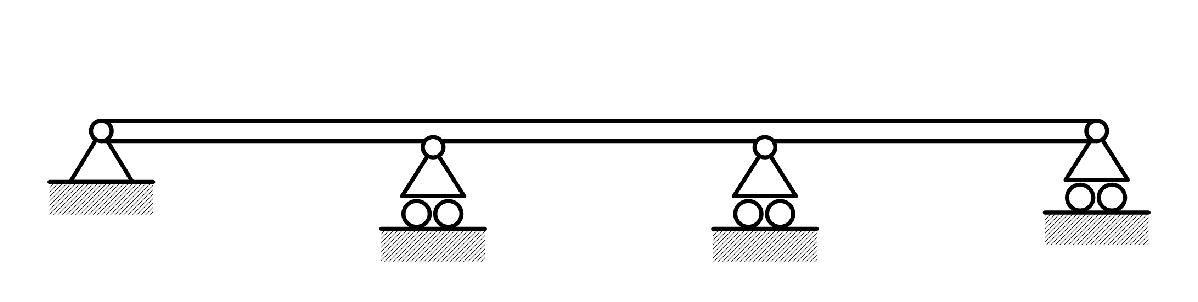
\includegraphics[width = \textwidth]{beam_model.pdf}
        \caption{连续梁模型}
    \end{subfigure}
    \caption{典型工程结构及其模型}
\end{figure}

\subsubsection{近代力学}

20世纪初,经典物理学面临着两大问题,其一是黑体辐射问题,由此产生了量子力学,其二是探讨光速不变的问题,由此产生了相对论。从此开始,物理学和力学之间出现了比较明显的界限。

\begin{figure}[ht]
    \centering
    \begin{subfigure}[t]{0.45\textwidth} \centering
        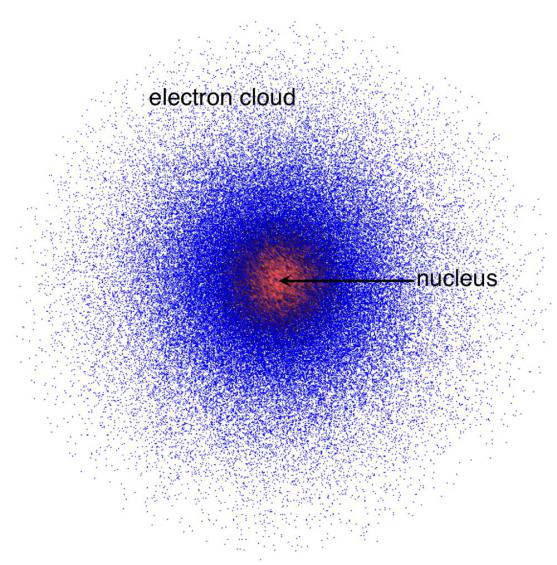
\includegraphics[height = 0.55\linewidth]{quantum.png}
        \caption{量子力学中的电子云图}
    \end{subfigure}\quad
    \begin{subfigure}[t]{0.45\textwidth} \centering
        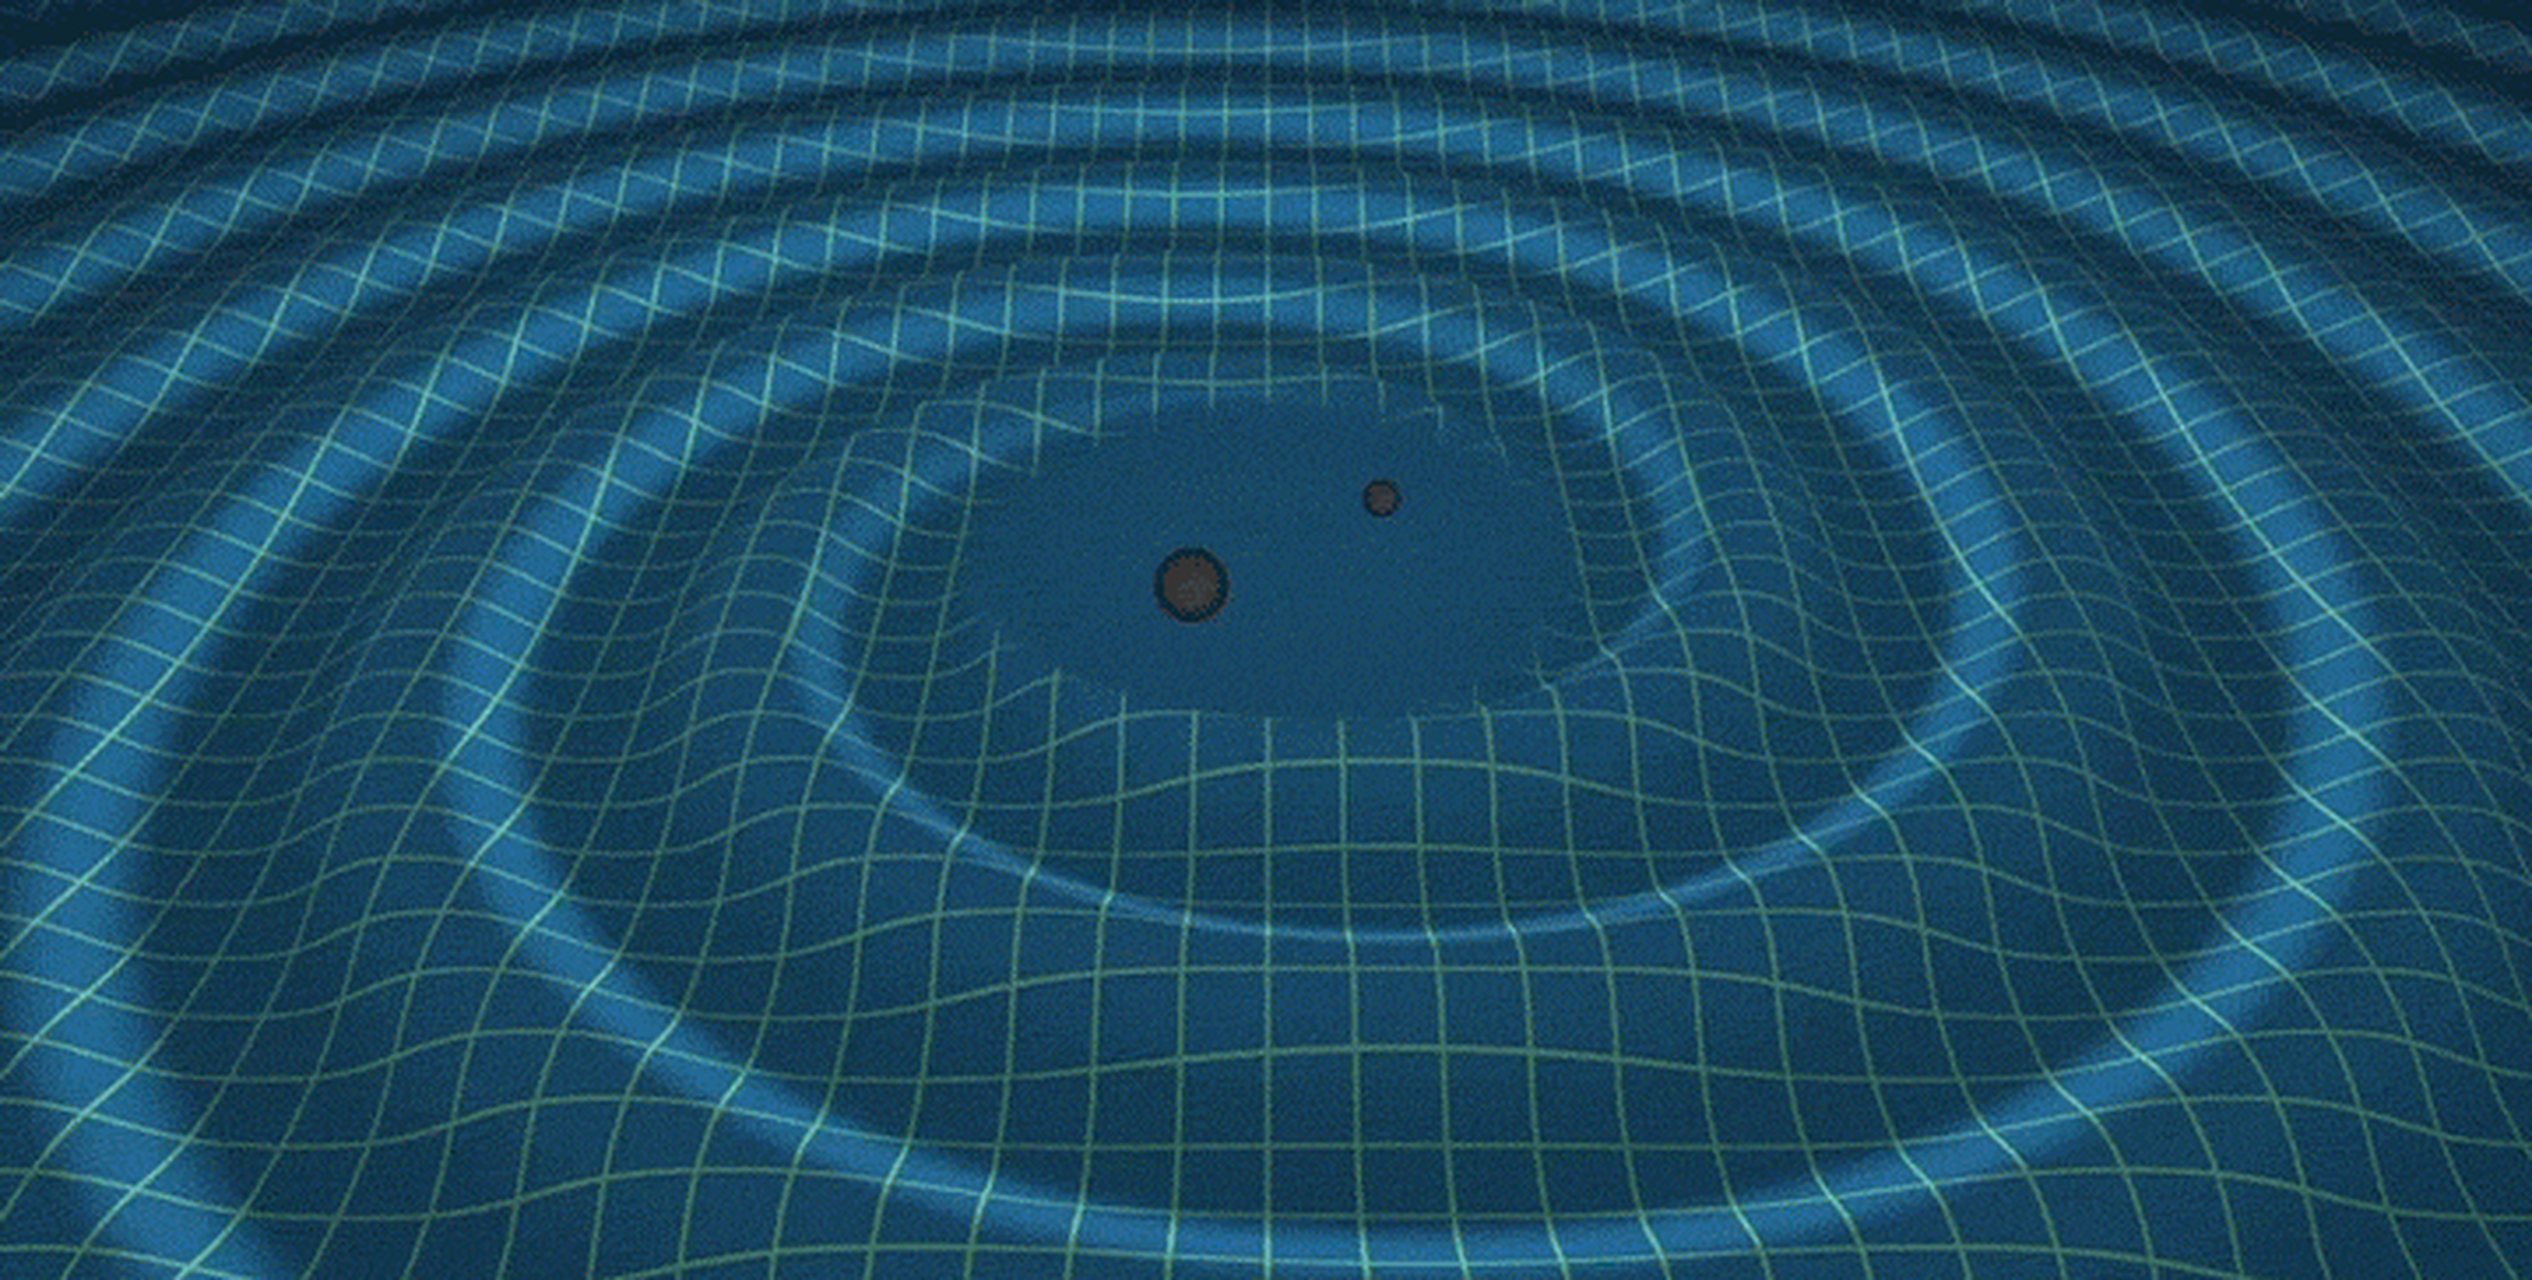
\includegraphics[height = 0.55\linewidth]{relativity.jpeg}
        \caption{广义相对论所预言的引力波现象}
    \end{subfigure}
\end{figure}

量子力学关心原子、分子尺度上基本粒子的性质,相对论则深入地考虑了我们所处宇宙的时空背景。这二者都是在不同情况下对经典力学的修正,经过适当的退化,它们可以分别得到经典力学中的结果。同时,经典力学能够足够精确地描述宏观、低速下的物理问题,而且这些问题还没有被完全解决,所以经典力学不仅没有走到尽头,反而得到进一步的发展,直至今天,形成了目前的力学这一学科。

时间来到20世纪,力学比较明显地分化出了“应用派”和“理论派”。这是由于,一方面理论物理的发展已经远远超过工程实践的能力,于是诸多工程内容需要依靠力学理论指导进行;另一方面,即使是经典力学中尚有诸多问题没有得到回答,有些知识更需要建立一个完善的体系。这种分化也不是20世纪才出现的,事实上早已有之,总有一些理论是比较超前的,暂时找不到它的用处,也有一些理论是为了解决当前的问题而提出的半经验或经验的模型,这就分别对应“理论派”和“工程派”。不过,这二者之间不是完全对立的关系,理论与实践是相辅相成的,只是二者之间分化的趋势到20世纪比以前更加明显了。目前,将力学与工程相结合是主要的趋势。

20世纪初这段时间的力学发展了以下主要内容:

一般力学中的许多问题最终都归结到求解常微分方程组中,不过解析求解一般的常微分方程组是困难的,于是人们便去研究方程的性质和行为。在研究非线性微分方程的过程中,陆续发现了周期解、非线性振动、分叉、混沌等现象,促进了微分方程定性理论的发展。

\begin{figure}[ht]
    \centering
    \begin{subfigure}[t]{0.45\textwidth} \centering
        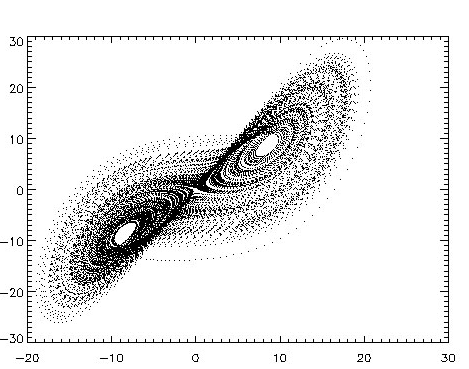
\includegraphics[height = 0.55\linewidth]{chao.jpeg}
        \caption{混沌现象中的奇异吸引子}
    \end{subfigure}\quad
    \begin{subfigure}[t]{0.45\textwidth} \centering
        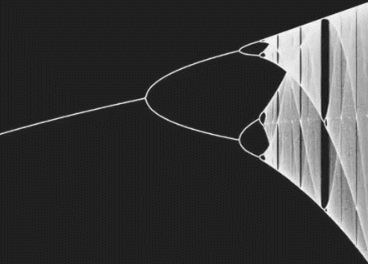
\includegraphics[height = 0.55\linewidth]{bifurcation.png}
        \caption{分叉现象}
    \end{subfigure}\bigskip

    \begin{subfigure}[t]{0.45\textwidth} \centering
        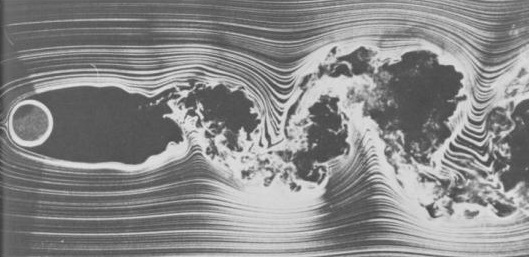
\includegraphics[height = 0.55\linewidth]{turbulent.jpeg}
        \caption{圆柱绕流产生的湍流现象}
    \end{subfigure}
\end{figure}


流体力学部分继续对N-S方程进行研究。N-S方程具有强烈的非线性,它具有描述湍流现象的能力,但求解是十分困难的。雷诺将速度写为平均速度与脉动速度之和,将压强写为平均压强与脉动压强之和,得到了平均意义下的N-S方程,后人称之为雷诺方程。\uwave{普朗特}、\uwave{冯·卡门}、\uwave{泰勒}、\uwave{周培源}、\uwave{柯尔莫哥洛夫}进一步做了一些工作,开创了湍流统计理论的研究。另一边,飞机的发明刺激了对机翼升力问题的研究,普朗特、\uwave{兰开斯特}、\uwave{芒克}等人合作建立了“升力线”理论,对翼型设计起到了指导作用。

\begin{marginparfigure}
    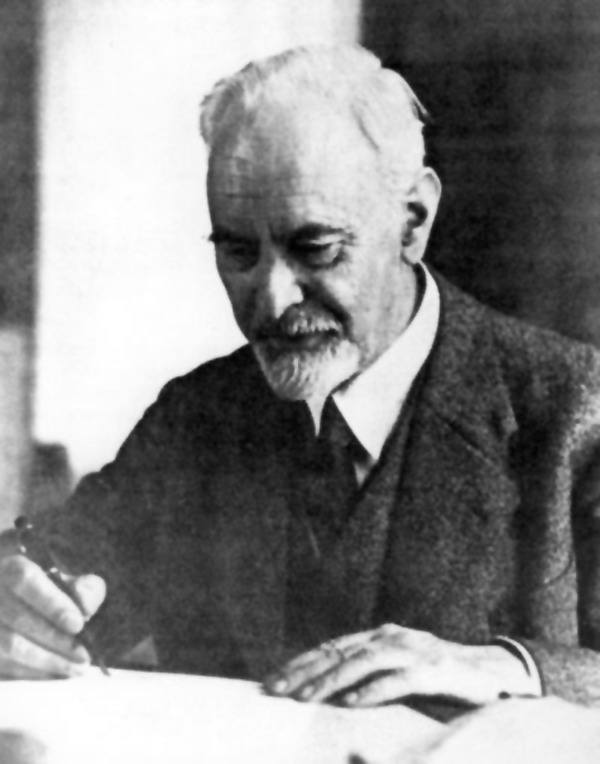
\includegraphics[width = 2.8cm]{Prandtl.jpeg}
    \captionof{figure}{普朗特像}
\end{marginparfigure}


\begin{marginparfigure}
    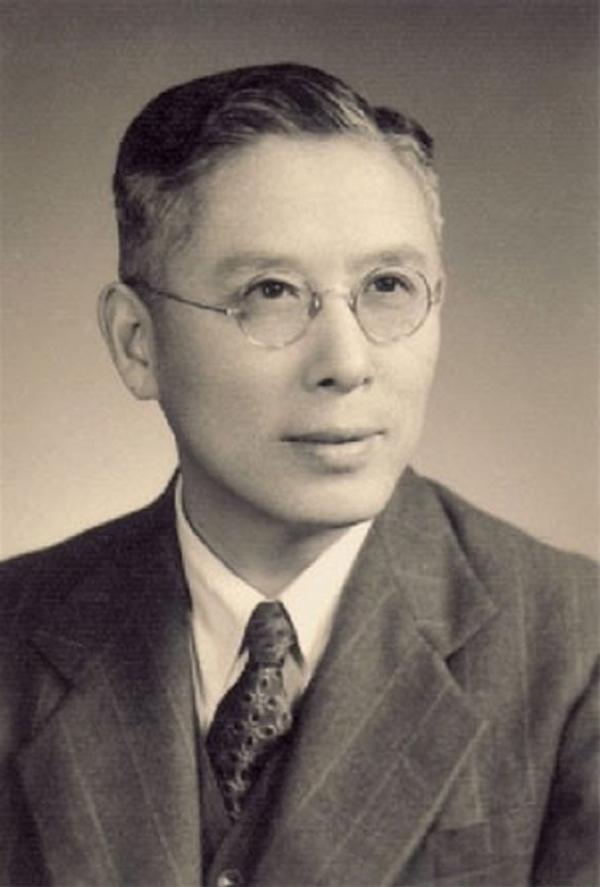
\includegraphics[width = 2.8cm]{Zhou.jpeg}
    \captionof{figure}{周培源像}
\end{marginparfigure}



\begin{figwindow}[0,r,
        {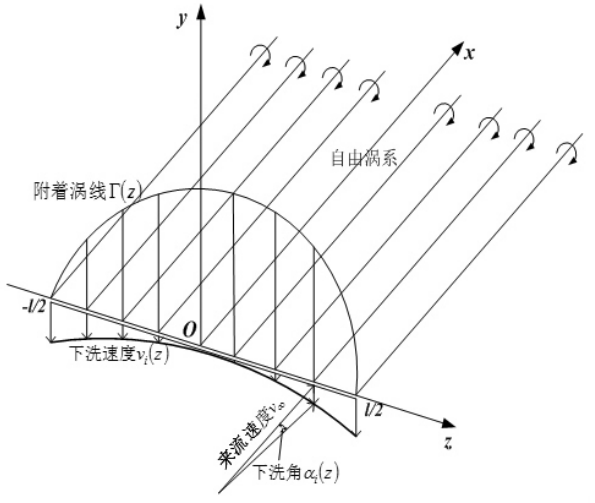
\includegraphics[width = 0.4\linewidth]{liftingline.png}},
        升力线模型]
    固体力学部分,人们已经将弹性理论中的大部分线性问题研究清楚了,这时开始考虑梁、板、壳等结构的稳定性,以及板壳的一般理论等。塑性力学、断裂力学以及疲劳问题等研究也已开始进行,就是说,这段时间的研究以及不再限于线弹性问题,而是向更多的非线性问题发起冲击。此外,麦克斯韦等考虑了黏弹性体模型,进而引发了人们对一般连续介质的性质的探讨,并最终形成了连续介质力学,并且促进了理性力学的复兴。
\end{figwindow}



此外值得一提的是计算机的发明导致了计算力学这一分支的产生。20世纪初,人们已经需要求解大规模复杂工程中的力学问题,但庞大的问题规模时代靠人力解决这些问题是极端困难的。计算机的问世和发展,强化了人类的计算能力,使得求解大规模力学问题成为可能。计算力学就是这样一门借助计算机解决力学问题、分析力学性质的学科,它处于力学、数学、计算机三门学科交叉的位置。计算力学当中的方法已经能够比较好地解决大部分线性问题,而对于数学本质是非线性的问题,如何用计算力学的手段去解决和分析还是很有挑战性的课题。

\begin{figure}
    \centering
    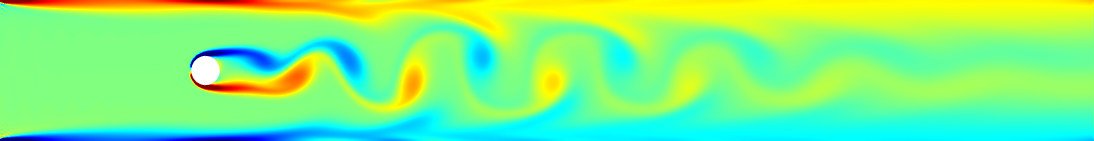
\includegraphics[width = \textwidth]{calculation_fluent.png}
    \caption{基于MATLAB编写的圆柱绕流涡量图计算结果}
\end{figure}

\begin{figure}
    \centering
    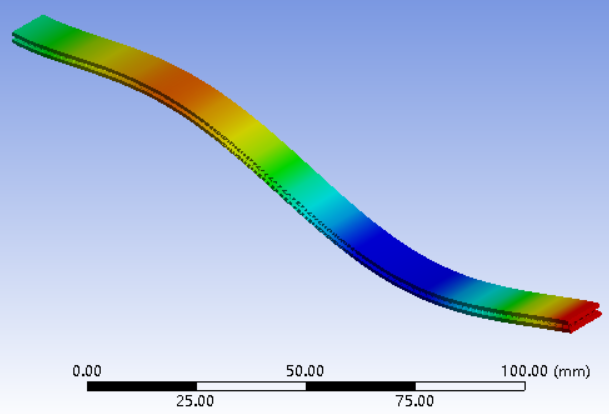
\includegraphics[scale=0.7]{calculation_solid.png}
    \caption{基于商业有限元软件ANSYS Workbench的悬臂梁自由振动位移云图}
\end{figure}

\subsection{力学的研究内容}

概括地说,力学是\textbf{研究宏观低速的物体机械运动规律的学问}。这一句话中包含了两个限定以及研究的对象。

\textbf{宏观},指的是忽略量子效应,而不一定是肉眼可见才叫宏观,有时,力学也会研究微纳米尺寸的问题,而不计量子效应的影响。\textbf{低速},指的是忽略相对论效应,天体力学能够解决太阳系范围内很多天体运动的问题,但在更大尺度的宇宙环境中,可能要考虑相对论效应的影响,这已经超出力学的研究范畴。总之,除了个别的极特殊情况,我们所讨论的力学都是经典范畴的。

\textbf{物体},其含义可以按照基于某种假设将实际物体抽象成的某种模型,再对这个模型加以研究。这些模型无外乎以下几种:\uwave{质点}、\uwave{刚体}、\uwave{连续介质}。

我们在中学阶段就学过了质点模型,这种模型假设忽略物体的尺寸大小,将物体视为有质量的点,例如,在考虑行星绕恒星运动时就会应用质点模型。

刚体则考虑了物体的尺寸、形状,但仍然认为物体是刚度无穷大的,也就是不会发生变形,准确的说法是“在物体上任取两点,这两点的距离是一个恒定值”。这种刚体模型相较于质点模型更加常见,杆、齿轮等机械构件在运动时,不可以忽略其形状因素,这时可以将它们视为刚体。

\begin{figwindow}[2,l,{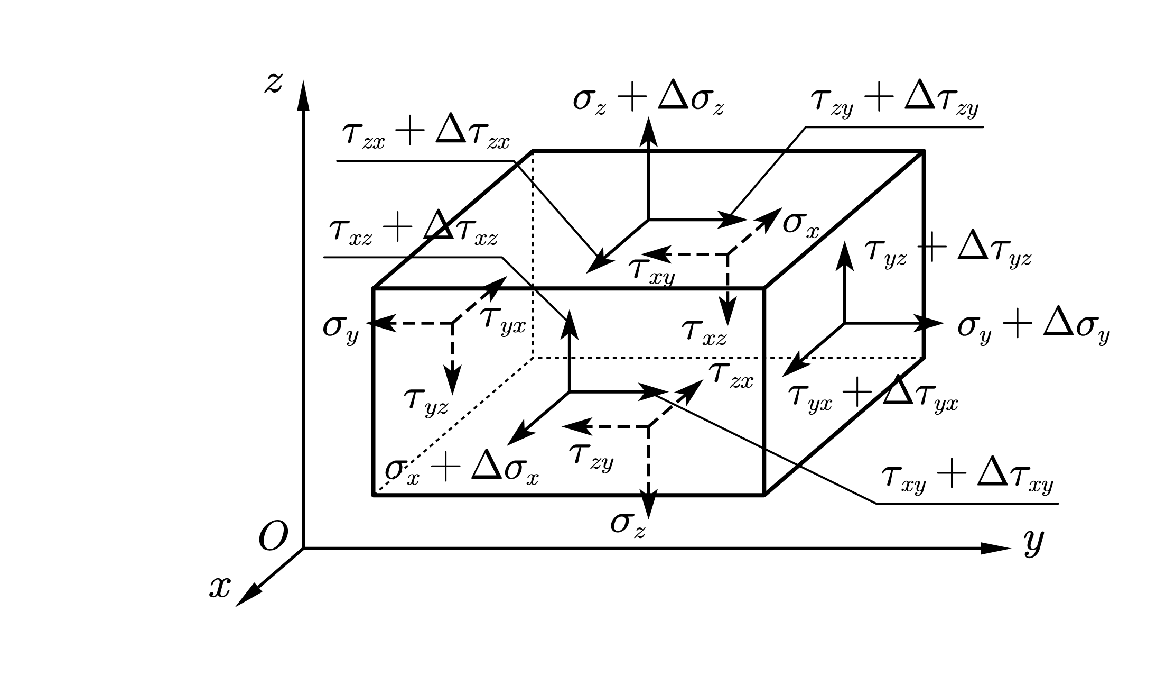
\includegraphics[width = 0.6\linewidth]{infinitesimal.pdf}},
        线弹性变形体微元的受力分析]
    连续介质是一个相当宽泛的模型,它可以涵盖多数固体、液体、气体。其最显著的特征是要考虑物体的变形。我们将etcounter这种模型称为“连续介质”的原因是,该模型的基本假设是“连续性假设”,即材质相同的一块物质是无限可分的,这样就可以应用微积分、场论等分析学工具对物体的变形加以研究。再根据物体变形的性质(可以理解为内力与变形及变形速率的关系)不同对其进行分类,粗略地讲,按照物体能否有效地抵抗剪切力将物体分为固体和流体,再按照流体是否可发生压缩变形分为气体和液体,按不同类别分别加以研究。例如,在研究杆、梁、轴的变形时,将它们视为固体;水是典型的液体,空气是典型的气体。
\end{figwindow}



\textbf{机械运动}是描述物体的空间位置随时间变化的过程,大致可分为\uwave{刚性运动}和\uwave{变形}。所谓刚性运动,即是指质点和刚体可以发生的机械运动,如平移、转动;而变形是物体的形状在外界作用下发生了变化,如弹簧的形变、弹性体的形变等。

我们首先对力学的研究范围做了一个大致限定,也了解了力学中的一些基本模型和概念。然而在某些必要的时候,可以适当放宽这些限制,力学的研究对象也可能随着科学技术的进一步发展而得到扩充。
目前,力学学科的二级分类大致就按照模型不同,分为\textbf{一般力学(与力学基础)}、\textbf{固体力学}和\textbf{流体力学},此外还有更加面向工程应用的\textbf{工程力学}和一些其他分支。下面,我们具体到目前力学学科的主要分支当中,看看不同力学分支的主要研究内容。

\subsubsection{一般力学与力学基础}

一般力学大致是动力学与控制的同义词,它的研究对象是宏观的离散力学系统和经典力学的一般原理。力学基础的对象比较广泛,但仍以离散系统为主。

\paragraph{天体力学}

天体力学是天文学和力学之间的交叉学科,研究对象小至太阳系内的天体,大至恒星系。其又下含几个次级学科,包括摄动理论、定性分析、数值计算、天体形状与自旋理论等,以及其他一些相对独立的课题。

\begin{figure}[ht]
    \centering
    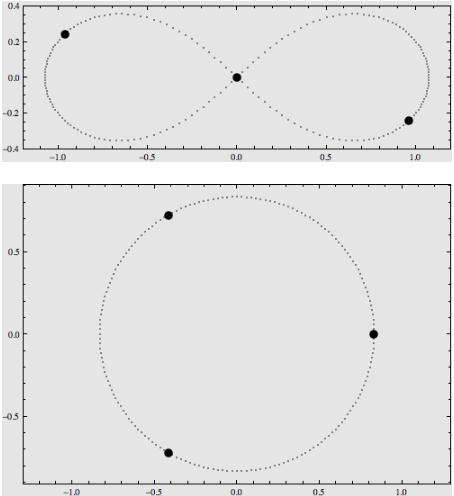
\includegraphics[scale=0.6]{three_bodies.jpeg}
    \caption{天体力学中的三体问题,两个特殊解}
\end{figure}

\paragraph{刚体动力学}

刚体动力学研究刚体在外力作用下的运动规律。它是计算机器部件的运动,舰船、飞机、火箭等航行器的运动以及天体姿态运动的力学基础。主要的次级研究内容有陀螺力学、转子动力学等。


\paragraph{分析力学}

分析力学通过用广义坐标为描述质点系的变量,运用数学分析的方法,研究宏观现
象中的力学问题。早期内容包括拉格朗日力学和哈密顿力学,后来又对有约束系统做了讨论。目前理论体系已经比较完备,主要考虑其具体应用。

\paragraph{运动稳定性}

运动稳定性研究物体或系统在外干扰的作用下偏离其原有运动后返回该运动的性质,对于运动稳定性的研究大都出于工程技术需要。奠定运动稳定性相关理论基础的是\uwave{庞加莱}和\uwave{李雅普诺夫}%
\begin{marginparfigure}
    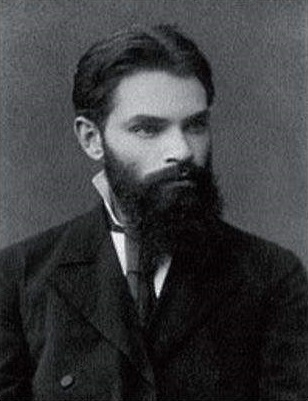
\includegraphics[width = 2.8cm]{Lyapunov.jpeg}
    \captionof{figure}{李雅普诺夫像}
\end{marginparfigure}%
,特别是李雅普诺夫开创的分析方法已经在诸多领域中得到应用。

\paragraph{非线性振动}

恢复力与位移不成正比或阻尼力不与速度一次方成正比的系统的振动都算是非线性振动。线性振动理论已经发展得比较完善,但在实际问题中,总有一些用线性理论无法解释的现象。一般来说,线性模型只适用于小运动范围,超出这一范围,按线性问题处理就会引起较大误差。

\begin{figure}
    \centering
    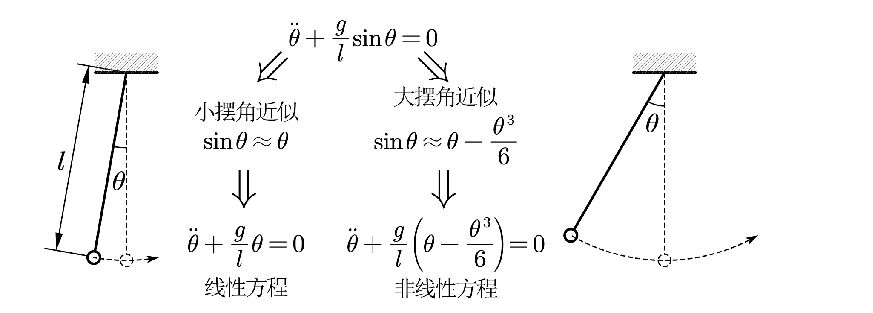
\includegraphics[width = 13cm]{pendulum.pdf}
    \caption{最简单的非线性振动的例子:大摆角单摆振动}
\end{figure}


\subsubsection{固体力学}

固体力学是力学当中成形较早、理论性和应用性都比较强的一个分支。它主要研究变形体在外界影响下内部发生的运动、变形等规律。固体力学当中的线弹性、小变形理论已经发展得相当完善,目前研究的方向多是非线性问题及随机性问题,典型的非线性问题有大变形、稳定性、断裂、疲劳、冲击等。


\begin{wrapfigure}[9]{r}{5cm}
    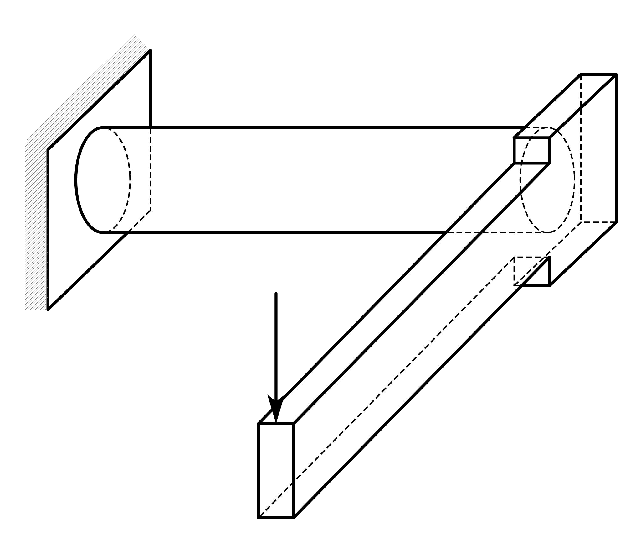
\includegraphics[width=5cm]{material_mechanics.pdf}
    \caption{材料力学中一个承受弯扭作用的结构件}
\end{wrapfigure}
\paragraph{材料力学} 材料力学主要研究简单结构件的变形、稳定性和强度问题。广泛地说,断裂、疲劳、强度、蠕变、试验测定等都可归入到材料力学的范畴。实际上,材料力学并不能算是一个独立的研究方向,它其实是在弹性力学获得结果的基础上,引入合理的假设,得到足够工程实用的结果。因此,材料力学更像是面向工程师的弹性力学简化版,或者作为入门固体力学时的学习材料。


\paragraph{结构力学}



结构力学研究的是杆、梁、\uwave{板}、\uwave{壳}等工程基本结构及其组合的变形和受力。结构力学由材料力学和弹性力学发展而来,主要研究内容有结构静力学、结构动力学、稳定性理论、断裂和疲劳。其中,结构静力学的发展比较成熟,并且由其中的“位移法”产生了计算力学的雏形。结构动力学研究的是在动态外载作用下结构的响应,主要围绕结构振动展开。稳定性理论、断裂和疲劳则是关注工程结构,而非一般的弹性体。

\begin{figure}[h]
    \centering
    \begin{subfigure}[t]{0.4\textwidth} \centering
        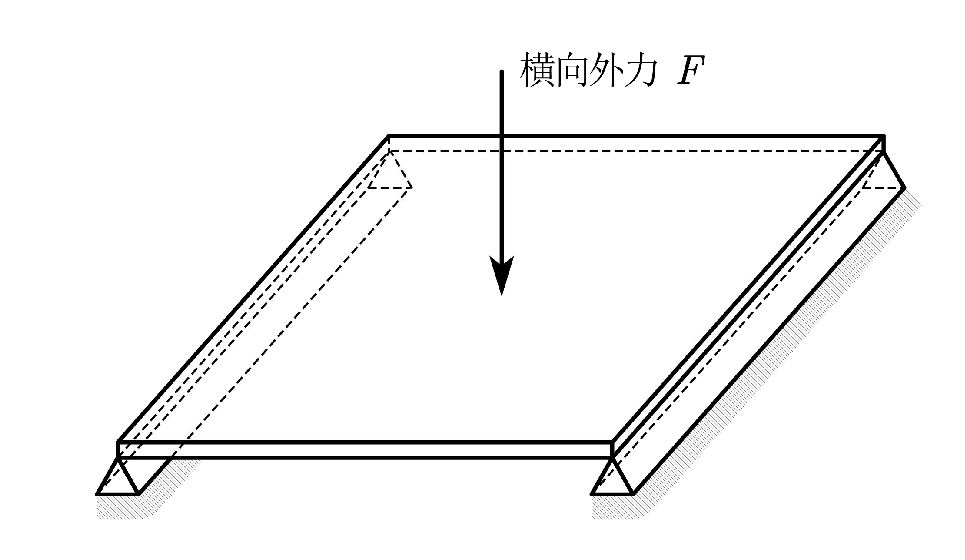
\includegraphics[height = 0.55\linewidth]{plate.pdf}
        \caption{两边简支薄板}
    \end{subfigure}\quad
    \begin{subfigure}[t]{0.4\textwidth} \centering
        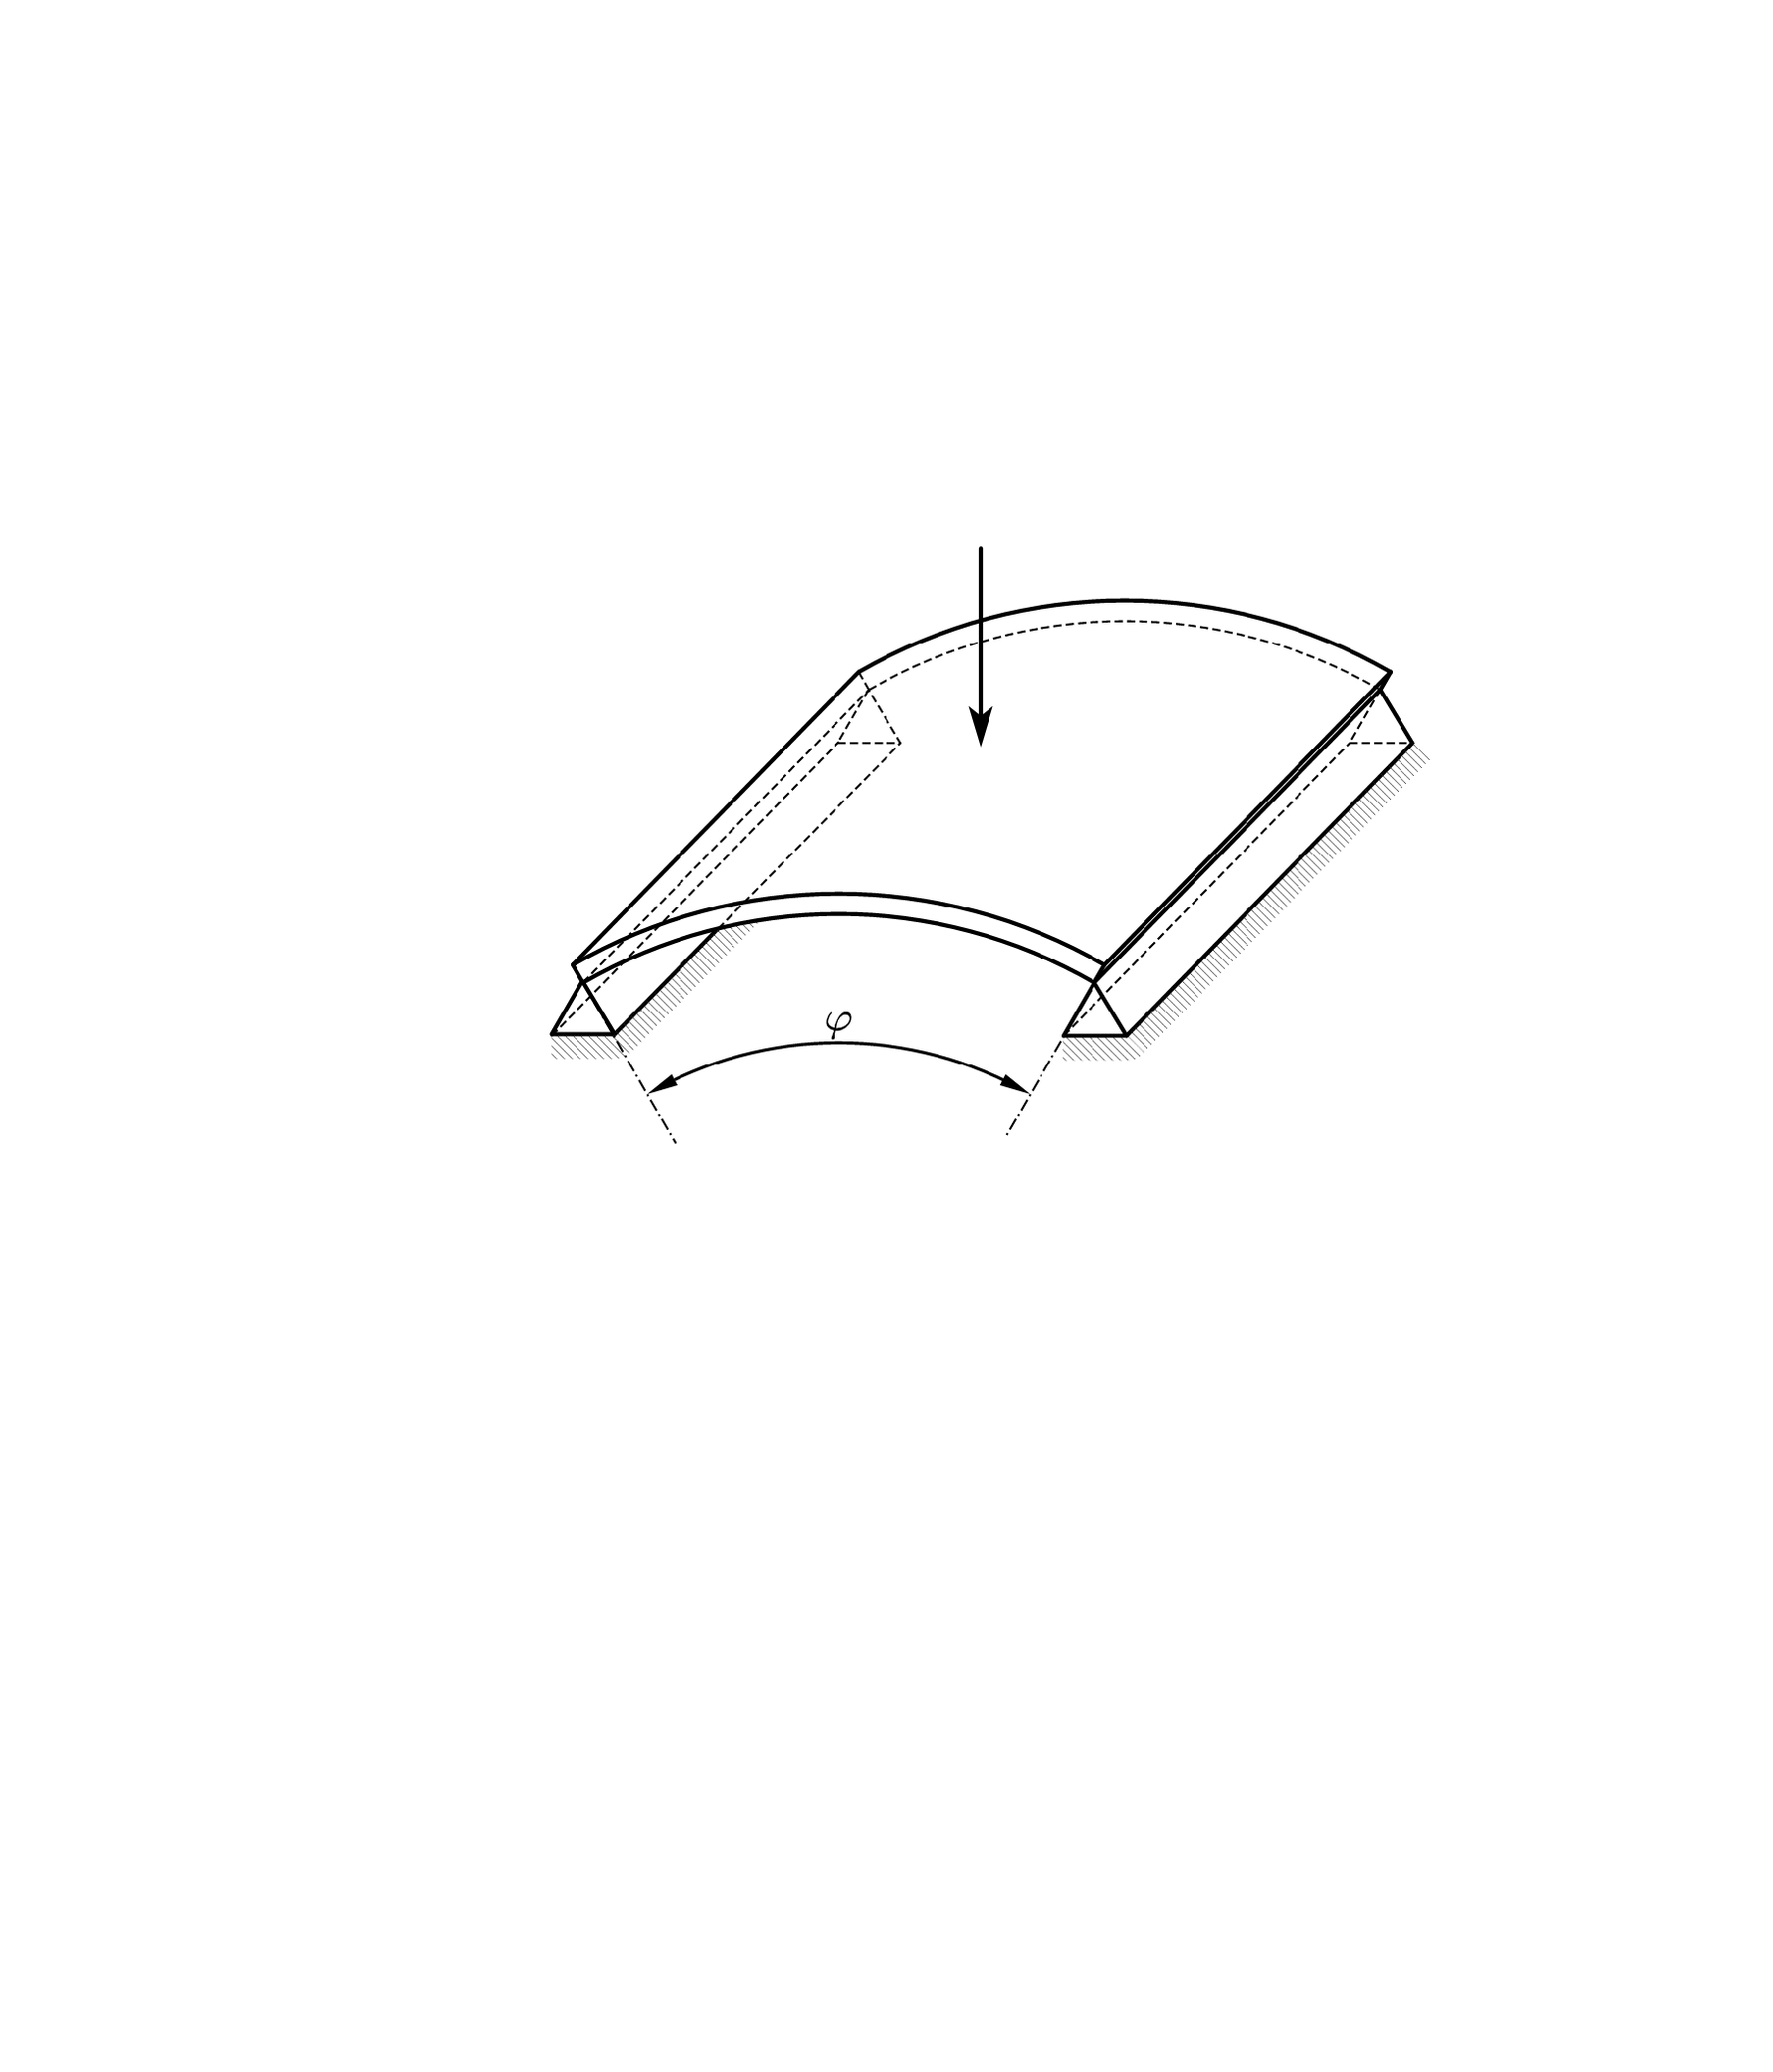
\includegraphics[height = 0.55\linewidth]{shell.pdf}
        \caption{两边简支圆柱薄壳}
    \end{subfigure}\bigskip
    \caption{板壳结构}
\end{figure}

\begin{marginpartext}
        板可以视作二维的梁,它同样主要承受横向外力。如果板足够薄,使得其几乎不能承受横向外力,就称其为膜。

        壳则是弯曲的板,由于几何形转是弯曲的,所以其受力平衡方程及动力学方程更加复杂。
\end{marginpartext}

\paragraph{弹性力学}

弹性力学是固体力学的基础,它研究一般弹性体在外载作用下的内力、变形情况。线弹性力学的基本理论早已建立,一些典型问题的解也已给出,也在此基础上分化出了材料力学和结构力学。目前,弹性力学有三个方向,第一个是与其他学科相互交叉,以研究多场作用耦合(如重力场、电磁场、化学场等多个场同时作用的力学系统)的力学模型;第二个是继续深化弹性力学的数学理论,研究非线性问题;第三个是研究弹性动力学理论,主要研究弹性体的振动及波的传播,这些内容在地震、地质勘探等领域有直接应用。

\paragraph{塑性力学}弹性体在受外力较小时,发生弹性变形,满足广义胡克定律,当弹性体受力超过其弹性极限后,其变形不再满足广义胡克定律,同时也会发生不可恢复的变形,这就是\uwave{塑性变形},而塑性力学就是研究弹性体发生塑性变形时,其变形与内力与外力之间关系的学科。塑性力学的主要研究内容有屈服条件、塑性增量理论和塑性本构关系。

\begin{figure}[h]
    \centering
    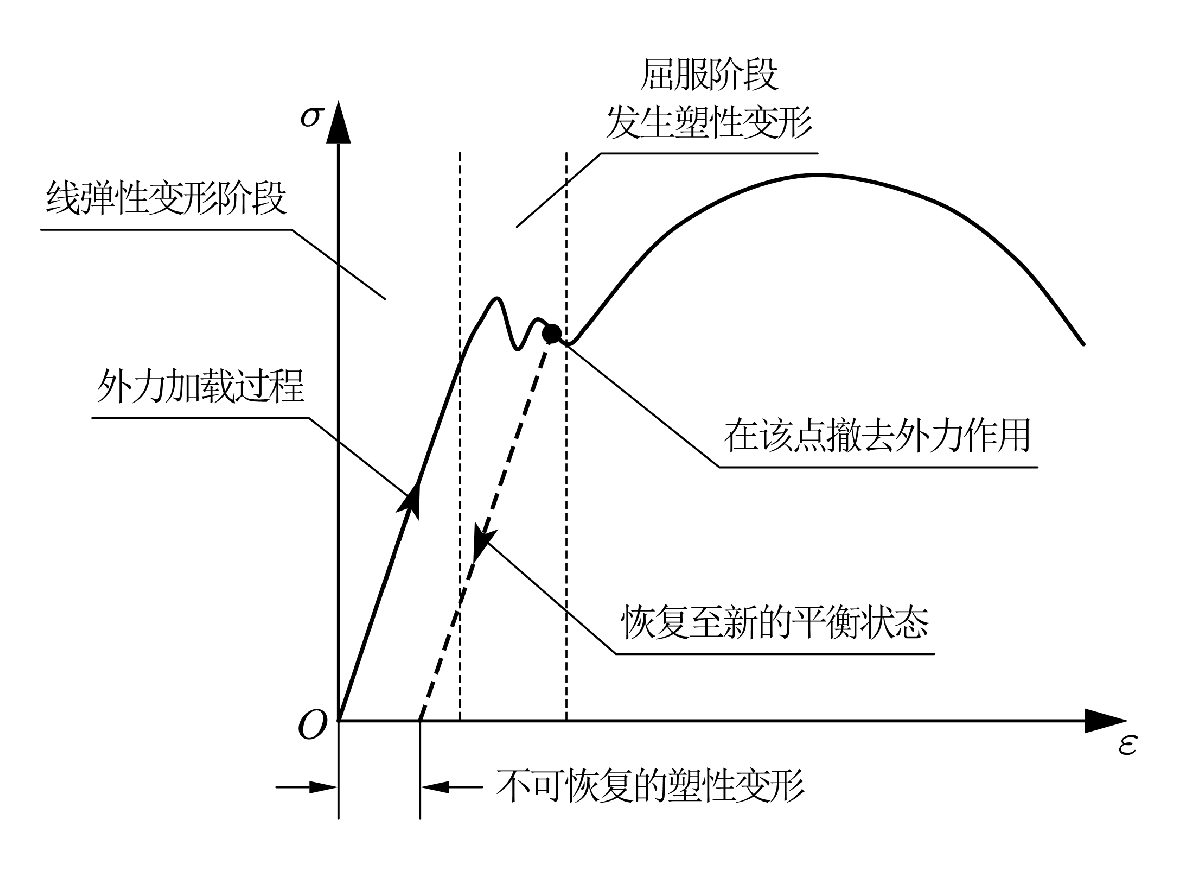
\includegraphics[width=9cm]{sigma_epsilon.pdf}
    \caption{塑性变形示意}
\end{figure}

\paragraph{断裂力学}

断裂力学是研究材料断裂失效和裂纹扩展规律的学科。该分支早期研究了裂纹扩展准则、裂纹尖端应力场分析、应力强度因子的计算方法等,以及如何将其应用到工程中去。目前的一些研究方面有:智能材料(压电、铁电等材料)的断裂与损伤、微纳米尺度断裂、非均质材料的断裂与损伤、断裂和损伤的试验与工程应用。

\begin{marginpartext}
        各向异性指的是某项物理规律与方向有关,同一位置处沿不同方向的物理规律不同。
\end{marginpartext}


\begin{wrapfigure}[8]{l}{5cm}
    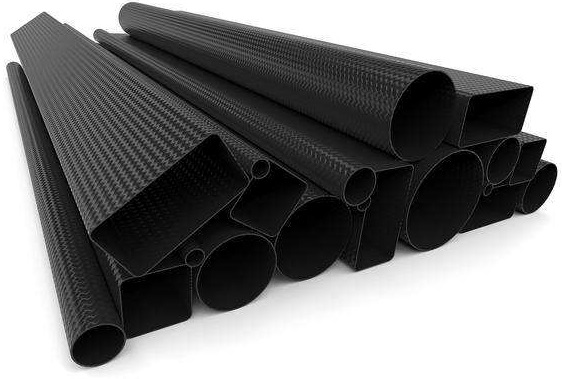
\includegraphics[width=5cm]{carbon_fiber.jpeg}
    \caption{碳纤维复合材料管}
\end{wrapfigure}

\paragraph{复合材料力学} \uwave{复合材料}是由两种或以上不同材料经过特定工艺复合而成的新型材料,其性能往往比传统材料更优,且具有良好的可设计性。宏观来看,复合材料最典型的特征是弹性规律的各向异性		,因此复合材料问题往往也具有一定的非线性。目前,复合材料力学主要研究以下几个方面:复合材料基础力学理论、纤维增强复合材料的细观力学、特种环境复合材料力学性能模拟表征与优化设计、功能梯度复合材料。



\subsubsection{流体力学}

流体力学主要研究流体(主要是液体及气体)在外力作用下发生的质量、动量、能量传输。

\begin{figure}
    \centering
    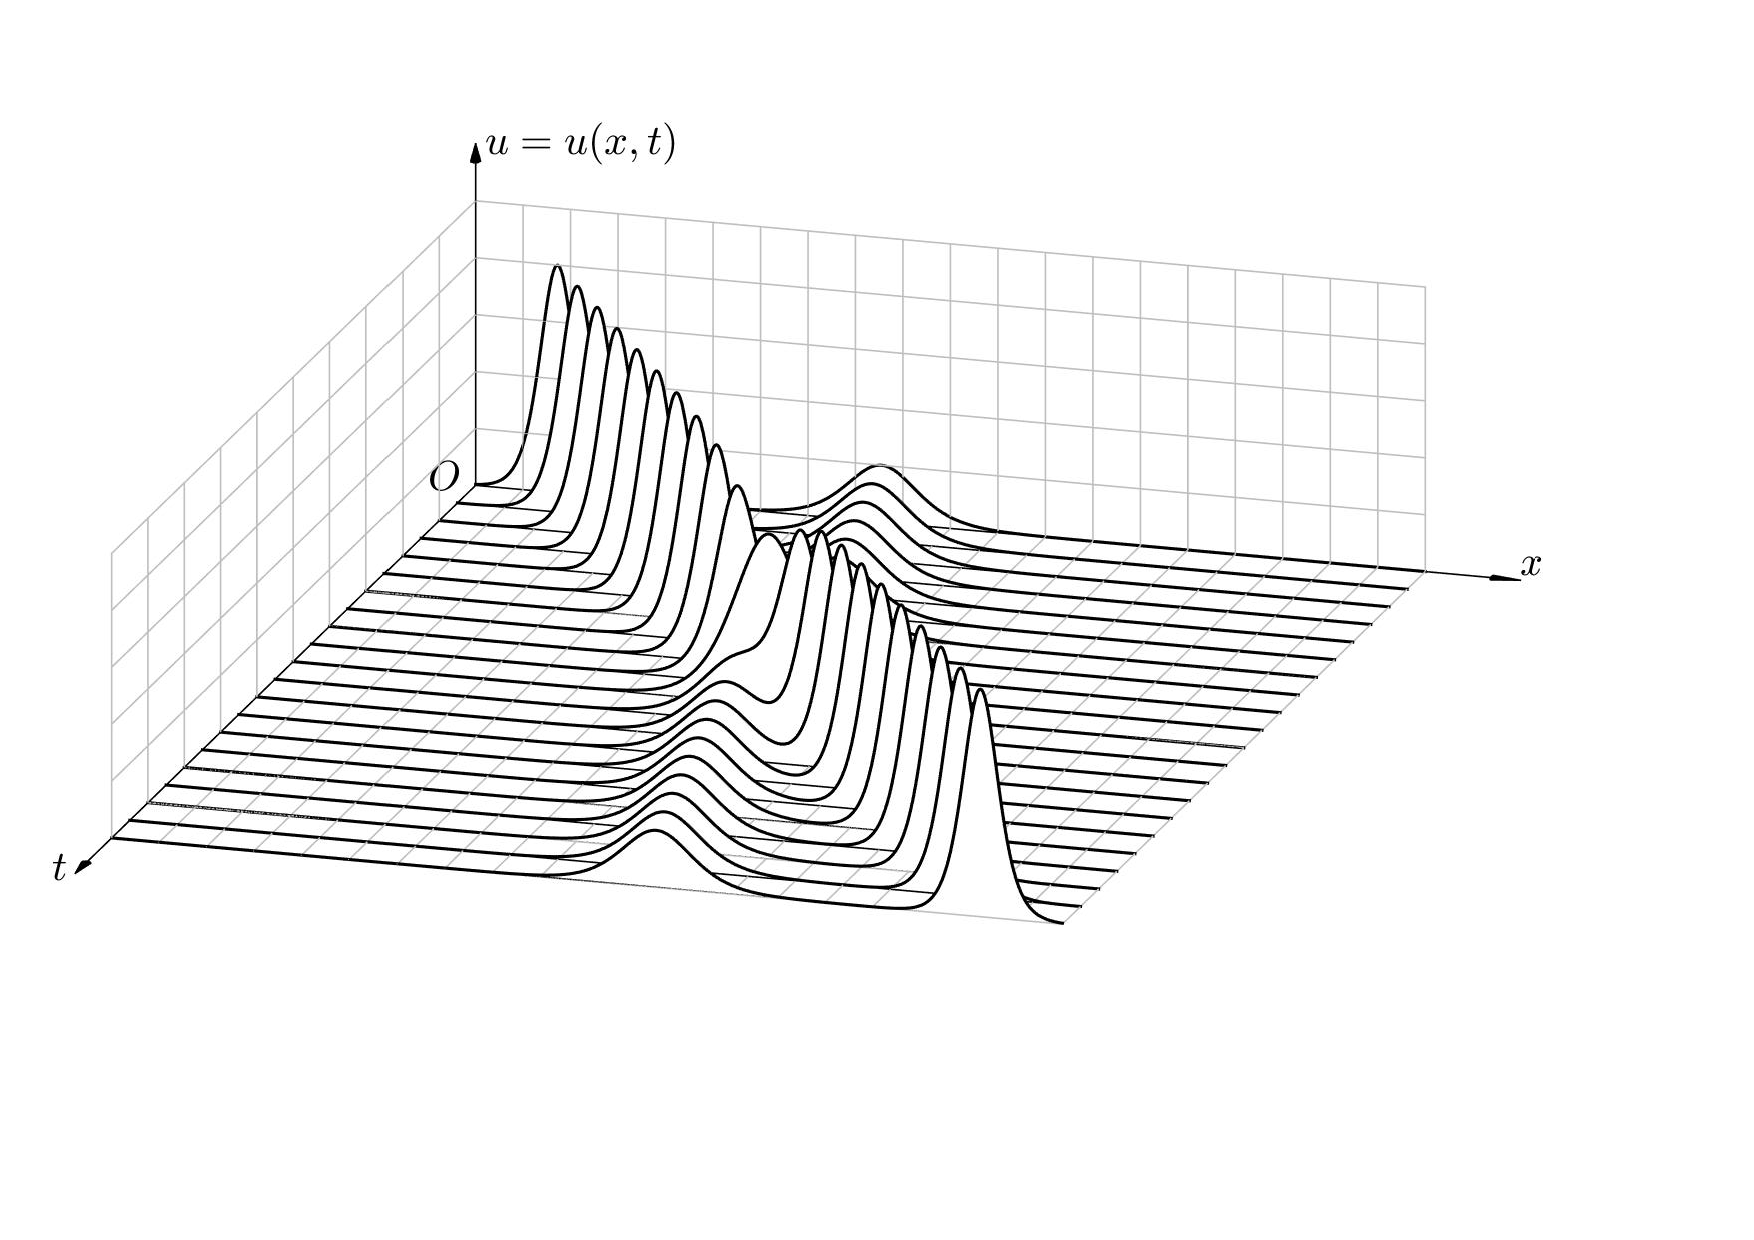
\includegraphics[scale=0.5]{solitary.pdf}
    \caption{两孤立波相作用的图像($x$-位置,$t$-时间,$u$-幅值)}
\end{figure}

\paragraph{理论流体力学}

流体力学的基本方程已经建立起来,但是其求解是十分困难的。流体力学的基本理论有理想流体力学、粘性流体力学、空气动力学。目前只研究清楚了一些特定流动形式,一般的流动、湍流现象还是很棘手的。此外,流体力学还研究非牛顿流体及其应用、孤立波等问题。总之,主要研究的是较复杂的非线性问题。

\paragraph{工程流体力学}

工程流体力学包括很多分支,如水力学、气动力学、渗流力学、多相流等问题,所研究的问题往往具有较强的非线性,直接求解十分困难,往往要借助新的数值手段和实验手段。

\subsubsection{其他分支}

力学领域还有许多分支,如计算力学,可以与上述几个大的方向相结合,去研究对应领域中的计算、仿真方法;再如工程力学,关心实际工程问题中的力学问题,注重应用各种力学手段去解决工程技术、制造当中的问题;又如理性力学,通过基本公理和数学原理推导力学知识体系,力求严密性。此外,还有许多新兴的领域,属于力学与其他学科交叉,例如生物力学、机器人动力学、地球力学、岩土力学等等,限于篇幅不一一介绍。

\subsection{力学的研究方法}

对于一般的自然科学来说,研究手段很多,但是力学的主要研究手段只有三项:理论分析、试验测试与数值方法。

\subsubsection{理论分析}

理论分析是力学学科的传统分析手段。从假设出发,利用数学工具,建立模型的控制微分方程及边界条件,或者是积分方程。如果能求得解析解,那么就将其解析解求出来之后分析,也可以直接进行分析。

理论分析是力学与数学联系最紧密的部分,一方面,数学当中的定量分析对于准确描述力学模型而言是极为有用的;另一方面,对力学模型的研究也促进着数学的发展,这一点从牛顿建立微积分来研究经典力学起就是这样了,直到今天。

\subsubsection{实验测试}

实验与测试是考察我们所建立力学模型究竟是否符合真实世界中物体运动规律的手段。目前,实验手段是多种多样的,机械测量、光测、电测等方法,并形成了专门研究实验方法与手段的实验力学。随着新技术的发展,还有新的测量手段与方法不断涌现出来。


\subsubsection{数值方法}

\begin{wrapfigure}{l}{5cm}
    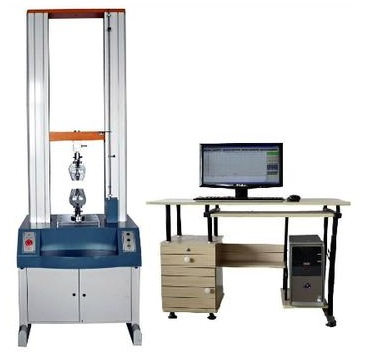
\includegraphics[width=5cm]{test.jpeg}
    \caption{测试试件基础力学性能的重要设备——万能试验机}
\end{wrapfigure}

数值方法是通过较为简单的代数运算方法,求出问题近似解的求解方法。一般来说,需要利用计算机进行辅助计算。

数值方法的主体就来自于计算力学,源自于早期的\uwave{有限差分法}(FDM)、瑞利-里兹法、伽辽金法,随着计算机的发展而兴盛起来,不断出现应用于各种问题的计算方法。目前,力学当中几乎各个领域的研究都离不开数值方法,数值仿真更是提供了一种节约成本的研究手段。对于一种数值计算方法,只有当其可靠性和效率都得到保证,才能算是成功的。一些比较成熟的数值仿真方法也已商用,在工程实践中发挥重大作用。例如,目前大多数商业计算力学软件中,处理固体力学问题的数值方法主要是基于\uwave{有限元法}(FEM)的,处理流体力学问题的数值方法主要是基于\uwave{有限体积法}(FVM)的。

\begin{figure}[ht]
    \centering
    \begin{subfigure}[t]{0.4\textwidth} \centering
        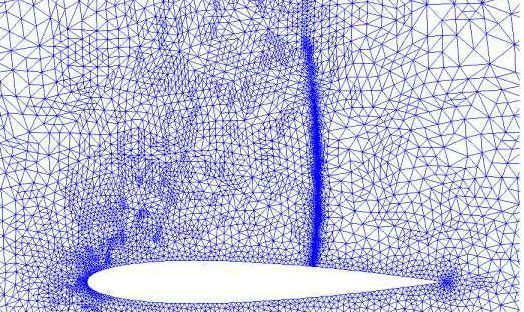
\includegraphics[height = 0.55\linewidth]{FVM.png}
        \caption{网格划分}
    \end{subfigure}\quad
    \begin{subfigure}[t]{0.4\textwidth} \centering
        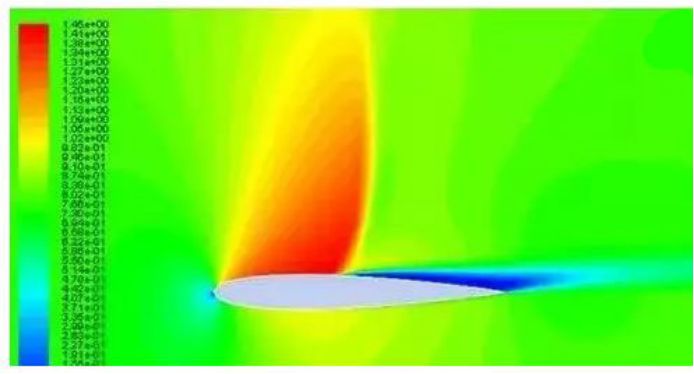
\includegraphics[height = 0.55\linewidth]{FVM_solution.png}
        \caption{计算结果}
    \end{subfigure}
    \caption{计算模拟机翼附近空气流动}
\end{figure}

另外,近年来以数据驱动的研究方法逐渐被力学研究者采用,有人主张将其归类为新的研究手段,但这里姑且也将其划到数值方法之中,因为这种方法也是基于数值处理的,且离不开计算机和人工智能技术的发展。数据驱动指的是从初始的数据或观测值出发,运用启发式规则,寻找和建立内部特征之间的关系,也指基于大规模统计数据的处理方法。力学当中主要使用的还是机器学习手段,目前,有学者用机器学习的方法研究一些流体问题。